%%%%%%%%%%%%%%%%%%%%%%%%%%%%%%%%%%%%%%%
%\clearpage
%\pagestyle{Ruled}
%%\chapterstyle{demo}
%\chapterstyle{veelo}
%%%%%%%%%%%%%%%%%%%%%%%%%%%%%%%%%%%%%%%%

\chapter{Miscellaneous} \label{chap:misc}

\setlength{\prechapterprecisshift}{-\onelineskip}

\chapterprecis{In which we talk of many things, but not shoes
               or ships or sealing wax, nor cabbages and kings.}

\noindent    This chapter started with the \cmd{\chapterprecis} command to add
the above text, which is also added to the \prtoc.

    The class provides a miscellany of minor facilities, which are described
here.

\section{Draft documents}

  The \Lopt{draft} option marks any overfull lines with black rectangles,
otherwise the appearance is the same as for a \Lopt{final} document.

\begin{syntax}
\piif{ifdraftdoc} \\
\end{syntax}
\glossary(ifdraftdoc)%
  {\cs{ifdraftdoc}}%
  {\ptrue\ if the \Popt{draft} class option has been used.}
The \piif{ifdraftdoc} macro is provided so that you can add extra
things that you might want to happen when processing a draft; for example
you might want to have each page header\index{header} (or footer\index{footer}) include the word `DRAFT'.
The code to do this can be put into a construct like the following:
\begin{lcode}
\ifdraftdoc
  % special things for a draft document
\else
  % perhaps special things for a non-draft document
\fi
\end{lcode}


\section{Change marks}

    When preparing a manuscript it normally goes through several iterations.
The macros described in this section can be used to identify changes made to 
a document throughout its lifecycle.

   The commands below implement a simplified version of the change
marking in the \Lclass{iso} class~\cite{ISOCLASS}.

\begin{syntax}
\cmd{\changemarks} \cmd{\nochangemarks} \\
\end{syntax}
\glossary(changemarks)%
  {\cs{changemarks}}%
  {Print change marks.}
\glossary(nochangemarks)%
  {\cs{nochangemarks}}%
  {Do not print change marks.}
The change marking macros only work properly when the \Lopt{draft} class
option is used. Additionally, the marks are only printed when the 
\cmd{\changemarks} declaration is in effect. Using \cmd{\nochangemarks}
switches off any marking.

\begin{syntax}
\cmd{\added}\marg{change-id} \\
\cmd{\deleted}\marg{change-id} \\
\cmd{\changed}\marg{change-id} \\
\end{syntax}
\glossary(added)%
  {\cs{added}\marg{change-id}}%
  {Change mark for someting added; \meta{change-id} is put in the margin.}
\glossary(deleted)%
  {\cs{deleted}\marg{change-id}}%
  {Change mark for someting deleted; \meta{change-id} is put in the margin.}
\glossary(changed)%
  {\cs{changed}\marg{change-id}}%
  {Change mark for someting changed; \meta{change-id} is put in the margin.}
Each of these macros puts a symbol and \meta{change-id} into the 
margin\index{margin} near
where the command is given. The \cmd{\added} macro indicates that something
has been added to the manuscript and uses $\oplus$ as its symbol. The
\cmd{\deleted} macro is for indicating that something has been deleted and uses
the $\neq$ symbol. The macro \cmd{\changed} uses the $\Leftrightarrow$ symbol
to indicate that something has been changed.

    These marking commands should be attached to some word or punctuation
mark in the text otherwise extraneous spaces may creep into the typeset
document.

\section{Trim marks}

    When the class \Lopt{showtrims} option is used, trim
marks can be placed on each page, usually to indicate where the stock should
be trimmed to obtain the planned page size. 

\begin{syntax}
\cmd{\showtrimsoff} \cmd{\showtrimson} \\
\end{syntax}
\glossary(showtrimsoff)%
  {\cs{showtrimsoff}}%
  {Switch off any trim marks.}
\glossary(showtrimson)%
  {\cs{showtrimson}}%
  {If the \Popt{showtrims} option has been used, switch on any trim marks 
  (this is the default).}
If the \Lopt{showtrims} class option has been used then the \cmd{\showtrimsoff}
declaration switches off the trim marks; the \cmd{\showtrimson} declaration,
which is the default, switches on the trim marks. These declarations do
nothing if the \Lopt{showtrims} option has not been used.

\LMnote{2013/05/01}{added caveat}
\begin{caveat}
  Most modern \LaTeX\ editors make use of the \emph{synctex} features
  in, say, pdf\LaTeX\ to enable \emph{reverse search} from the PDF
  previewer back to the source code in the editor. That is, click in a
  certain manner in the PDF previewer and you will be taken to the
  corresponding (or there about) line in the source code.

  Apparently the \emph{synctex} feature does not like the trimmarks
  the class provide, or the \pstyle{showlocs} page style. The code
  line one is referred back to may be off by tens of lines.

  Currently, there is no known workarounds for this deficiency.
\end{caveat}



    Trim marks can be placed at each corner of the (trimmed) page, and also
at the middle of each side of the page.

\begin{syntax}
\cmd{\trimXmarks} \\
\cmd{\trimLmarks} \\
\cmd{\trimFrame} \\
\cmd{\trimNone} \\
\cmd{\trimmarkscolor} \\
\end{syntax}
\glossary(trimXmarks)%
  {\cs{trimXmarks}}%
  {Trim marks of crosses at the four corners of the trimmed page.}
\glossary(trimLmarks)%
  {\cs{trimLmarks}}%
  {Trim marks of `L' shapes at the four corners of the trimmed page.}
\glossary(trimFrame)%
  {\cs{trimFrame}}%
  {Trim mark of a frame drawn round the trimmed page boundary.}
\glossary(trimNone)%
  {\cs{trimNone}}%
  {No trim marks.}
\glossary(trimmarkscolor)%
  {\cs{trimmarkscolor}}%
  {Empty macro that can be redefined to give a specific color to the trimmarks.}

Some predefined trimming styles are provided. After the declaration
\cmd{\trimXmarks} marks in the shape of a cross are placed at the four
corners of the page. The declaration \cmd{\trimLmarks} calls for corner marks
in the shape of an `L', in various orientations depending on the particular
corner. After \cmd{\trimFrame} a frame will be drawn around each page, 
coinciding with the page boundaries. The declaration \cmd{\trimNone}
disables all kinds of trim marking. All three plus \cs{quarkmarks}
(described below) is visibly shown on \fref{fig:trimmarks}.

The macro \cs{trimmarkscolor} is despite its name a normal (empty)
macro. By redefining it one can change the color of the trimmarks,
handy for example if the document has a dark background color. To make
them blue use
\begin{lcode}
\newcommand*{\trimmarkscolor}{\color{blue}}
\end{lcode}


\begin{syntax}
\cmd{\trimmarks} \\
\cmd{\tmarktl} \cmd{\tmarktr} \cmd{\tmarkbr} \cmd{\tmarkbl} \\
\cmd{\tmarktm} \cmd{\tmarkmr} \cmd{\tmarkbm} \cmd{\tmarkml} \\
\end{syntax}
\glossary(trimmarks)%
  {\cs{trimmarks}}%
  {Displays 8 (in)visible trim marks round the boundary of the trimmed page.}
\glossary(tmarktl)%
  {\cs{tmarktl}}%
  {Trim mark for top left of trimmed page.}
\glossary(tmarktm)%
  {\cs{tmarktm}}%
  {Trim mark for top middle of trimmed page.}
\glossary(tmarktr)%
  {\cs{tmarktr}}%
  {Trim mark for top right of trimmed page.}
\glossary(tmarkmr)%
  {\cs{tmarkmr}}%
  {Trim mark for middle right of trimmed page.}
\glossary(tmarkbr)%
  {\cs{tmarkbr}}%
  {Trim mark for bottom right of trimmed page.}
\glossary(tmarkbm)%
  {\cs{tmarkbm}}%
  {Trim mark for bottom middle of trimmed page.}
\glossary(tmarkbl)%
  {\cs{tmarkbl}}%
  {Trim mark for bottom left of trimmed page.}
\glossary(tmarkml)%
  {\cs{tmarkml}}%
  {Trim mark for middle left of trimmed page.}
\glossary(tmarktl)%
  {\cs{tmarktl}}%
  {Trim mark for top left of trimmed page.}
The \cmd{\trimmarks} macro is responsible for displaying up to 8 marks. The
marks are defined as zero-sized pictures which are placed strategically
around the borders of the page. 

    The command \cmd{\trimmarks} places the pictures \cmd{\tmarktl}, 
\cmd{\tmarktr},
\cmd{\tmarkbl}, and \cmd{\tmarkbr} at the top left, top right,
bottom right and bottom left corners of the page. The pictures
\cmd{\tmarktm}, \cmd{\tmarkmr}, \cmd{\tmarkbm}, and \cmd{\tmarkml} are placed
at the top middle, middle right, bottom middle and middle left of the
edges of the page. All these \verb?\tmark..? macros should expand to zero-sized
pictures.

\begin{syntax}
\cmd{\trimmark} \\
\end{syntax}
\glossary(trimmark)%
  {\cs{trimmark}}%
  {Cross mark used by \cs{trimXmarks}.}
The declaration \cmd{\trimXmarks} uses \cmd{\trimmark} for the corner 
crosses. This is defined as
\begin{lcode}
\newcommand{\trimmark}{%
  \begin{picture}(0,0)
    \setlength{\unitlength}{1cm}\thicklines
    \put(-2,0){\line(1,0){4}}
    \put(0,-2){\line(0,1){4}}
  \end{picture}}
\end{lcode}
which produces a zero-sized picture of a 4cm cross. Then \cmd{\trimXmarks}
is defined as:
\begin{lcode}
\newcommand*{\trimXmarks}{%
  \let\tmarktl\trimmark
  \let\tmarktr\trimmark
  \let\tmarkbr\trimmark
  \let\tmarkbl\trimmark}
\end{lcode}


    As an example, to draw short lines marking the half-height of the page, 
try this:
\begin{lcode}
\renewcommand*{\tmarkml}{%
  \begin{picture}(0,0)%
    \unitlength 1mm
    \thinlines
    \put(-2,0){\line(-1,0){10}}
  \end{picture}}
\renewcommand*{\tmarkmr}{%
  \begin{picture}(0,0)%
    \unitlength 1mm
    \thinlines
    \put(2,0){\line(1,0){10}}
  \end{picture}}
\end{lcode}
Thin horizontal lines of length 10mm will be drawn at the middle left and
middle right of the page, starting 2mm outside the page boundary. This
is what we do (now) by default for all four middle parts.


\begin{syntax}
\cmd{\quarkmarks} \\
\cmd{\registrationColour}\marg{mark} \\
\end{syntax}
\glossary(quarkmarks)%
  {\cs{quarkmarks}}%
  {Trim marks in the style of Quark Xpress registration marks, typeset with
   \cs{registrationColour}.}
\glossary(registrationColour)%
  {\cs{registrationColour}\marg{mark}}%
  {Typesets \cs{quarkmarks}.}
Following the declaration \cmd{\quarkmarks} and trim marks will be in
the style of Quark Xpress registration marks.\footnote{The code for this
was donated by William Adams\index{Adams, William}.} The marks will be
typeset using \cmd{\registrationColour}. The default definition is simply
\begin{lcode}
\newcommand*{\RegistrationColour}[1]{#1}
\end{lcode}
but you can change that to, say, print the marks in particular
color. See \fref{fig:trimmarks}.


\begin{figure}[htbp]
  \centering
  \ifpdf%
  \subbottom[\cs{trimXmarks}
  (default)]{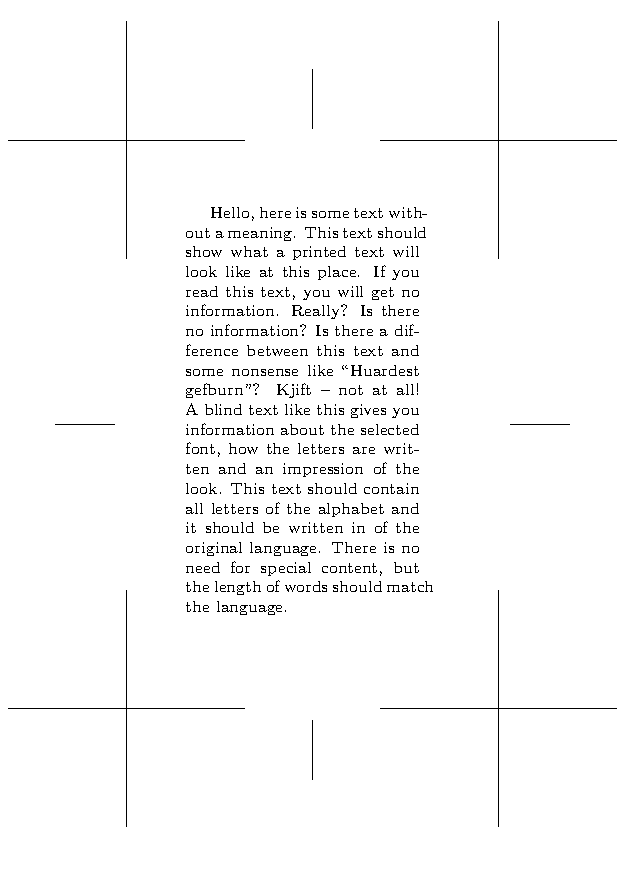
\includegraphics[page=1,scale=0.5]{trims-example}}
  \qquad\qquad
  \subbottom[\cs{trimLmarks}]{\includegraphics[page=2,scale=0.5]{trims-example}}
  \\%
  \subbottom[\cs{trimFrame}]{\includegraphics[page=3,scale=0.5]{trims-example}}
  \qquad\qquad
  \subbottom[\cs{quarkmarks}]{\includegraphics[page=4,scale=0.5]{trims-example}}
  \else%
  \texttt{examples only inserted in pdf-mode, now we can write and
    work in DVI-mode, /daleif}
  \fi%
  \caption{The four trimmark types}
  \label{fig:trimmarks}
\end{figure}





\section{Sheet numbering}

    One purpose of trim marks is to show a printer where the stock
should be trimmed. In this application it can be useful to also note the
sheet number on each page, where the sheet number is 1 for the first page 
and increases by 1 for each page thereafter. The sheet number is independent
of the page number.

\begin{syntax}
\Icn{sheetsequence} \\
\cmd{\thesheetsequence} \\
\end{syntax}
\glossary(sheetsequence)%
  {\Pcn{sheetsequence}}%
  {Counter for sheets (similar to \Pcn{page} for pages).}
\glossary(thesheetsequence)%
  {\cs{thesheetsequence}}%
  {Typesets the current sheet sequence number.}
The macro \cmd{\thesheetsequence} typesets the current sheet sequence number
and is analogous to the \cmd{\thepage} macro.

\begin{syntax}
\Icn{lastsheet} \\
\Icn{lastpage} \\
\end{syntax}
\glossary(lastsheet)%
  {\Pcn{lastsheet}}%
  {Counter holding the number of sheets processed during the \emph{previous}
   \ltx\ run.}
\glossary(lastpage)%
  {\Pcn{lastpage}}%
  {Counter holding the number of the last page processed during the \emph{previous}
   \ltx\ run.}
The counter \Icn{lastsheet} holds the number of sheets processed during
the \emph{previous} run of LaTeX. Similarly, the counter \Icn{lastpage}
holds the number of the last page processed during the previous run.
Note that the last page number is not necessarily the same as the last
sheet number. For example: \\
\textit{In this document this is 
        sheet \thesheetsequence\ of \thelastsheet\ sheets, 
        and page \thepage\ of \thelastpage.}

The previous sentence was the result of processing the following
code 
\begin{lcode}
\textit{In this document this is 
        sheet \thesheetsequence\ of \thelastsheet\ sheets, 
        and page \thepage\ of \thelastpage.}
\end{lcode}

    You may wish to use the sheet and/or page numbers as part of some
trim marks. The following will note the sheet numbers above the page.
\begin{lcode}
\newcommand*{\trimseqpage}{%
  \begin{picture}(0,0)
    \unitlength 1mm
    \put(0,2){\makebox(0,0)[b]{Sheet: \thesheetsequence\ of \thelastsheet}}
  \end{picture}}
\let\tmarktm\trimseqpage
\end{lcode}

\section{Gatherings or signatures}

    Sometimes publishers request that they be supplied with a total number of
pages that meet their planned \emph{gatherings}\index{gathering}.\footnote{There
was a thread on \ctt, \textit{pagenumber mod 4?} about this in 2008.}
 For instance
a gathering may consist of 8 leaves, and as there are two pages to a leaf this
is equivalent to 16 pages. To meet this particular requirement there must be 
a total of $8N$ leaves, or equivalently $16N$ pages, where $N$ will be 
the number of gatherings.

\begin{syntax}
\cmd{\leavespergathering}\marg{num} \\
\end{syntax}
\glossary(leavespergathering)%
  {\cs{leavespergathering}\marg{num}}%
  {Ensure that the correct number of pages are output to make up gatherings 
   of \meta{num} leaves each.}
The command \cmd{\leavespergathering} ensures that there will be exactly the
right number of pages output to make a complete set of gatherings of \meta{num}
leaves (2\meta{num} pages) each --- if necessary  blank pages will be output 
at the end to make up the correct tally. If \meta{num} is less than two (the default)
then no additional pages will be output.


\section{Time}

\begin{syntax}
\cmd{\printtime} \cmd{\printtime*} \\
\cmd{\hmpunct} \cmd{\amname} \cmd{\pmname} \\
\end{syntax}
\glossary(printtime)%
  {\cs{printtime}}%
  {Prints the time of day using a 24 hour clock.}
\glossary(printtime*)%
  {\cs{printtime*}}%
  {Prints the time of day using a 12 hour clock.}
\glossary(hmpunct)%
  {\cs{hmpunct}}%
  {Punctuation between hours and minutes in \cs{printtime} (default :)}
\glossary(amname)%
  {\cs{amname}}%
  {Abbreviation for ante meridiem used in \cs{printtime*} (default am)}
\glossary(pmname)%
  {\cs{pmname}}%
  {Abbreviation for post meridiem used in \cs{printtime*} (default am)}

The \cmd{\printtime} command\footnote{I based the code on a similar macro
in \btitle{\tx\ for the Impatient}~\cite{IMPATIENT}.} 
prints the time of day when the document is 
processed using the 24 hour clock while \cmd{\printtime*} uses a 12
hour clock. For example, the effect of the 
next piece of code is shown below.
\begin{lcode}
This document was processed on: \today\ at \printtime\ (\printtime*).
\end{lcode}
This document was processed on: \today\ at \printtime\ (\printtime*).

    The punctuation between the hours and minutes is \cmd{\hmpunct} which
defaults to a colon (:). The macros \cmd{\amname} and \cmd{\pmnane} hold 
the abbreviations for \textit{ante meridiem} and \textit{post meridiem}, 
respecitively; the defaults are `\amname' and `\pmname'. 

    According to the \btitle{Chicago Manual of Style}~\cite{CMS} there 
should be no punctuation between the hours and minutes in the 24 hour system.
For the 12 hour system it recommends that small caps be used for the
divisions of the day (e.g., \textsc{a.m.} and \textsc{p.m.}) and also
that the American practice is to use a colon as the separator between
hours and minutes whereas the English practice is to use a period (known
to the English as a `full stop'). I don't know what the traditions are
in other orthographies.

    The \cmd{\quarkmarks} declaration uses \cmd{\printtime}, so be careful
if you change it.

    Nicola Talbot's \Lpack{datetime} package~\cite{DATETIME} provides
a much more comprehensive collection of styles for printing the time;
also for dates.

\section{Page breaks before lists}

   A sentence or two may be used to introduce a list (e.g., \Ie{itemize})
and it can be annoying if there is a page break between the introductory words
and the first item.
\begin{syntax}
\cmd{\noprelistbreak} \\
\end{syntax}
\glossary(noprelistbreak)%
  {\cs{noprelistbreak}}%
  {Putting this immediately before an \Pe{itemize} (or \Pe{enumerate}, or \ldots) 
   environment should prevent a pagebreak.}

Putting \cmd{\noprelistbreak} immediately before the \verb?\begin{itemize}?
should prevent a page break. Ideally, there should be no blank lines
between the end of the introduction and the start of the list. 

\section{Changing counters}

    This is effectively a bundling of the \Lpack{chngcntr} 
package~\cite{CHNGCNTR}.

\begin{syntax}
\cmd{\newcounter}\marg{ctr}\oarg{within} \\
\cmd{\thectr} \\
\end{syntax}
\glossary(newcounter)%
  {\cs{newcounter}\marg{ctr}\oarg{within}}%
  {Creates a new counter \Pcn{ctr}, optionally reset when counter \Pcn{within}
   changes.}
\glossary(thectr)%
  {\cs{thectr}}%
  {Typesets the value of the counter \Pcn{ctr}.}
    In \ltx\ a new counter called, say \Pcn{ctr}, is created by the 
\cmd{\newcounter} command as \verb?\newcounter{ctr}?. 
If the optional \meta{within}
argument is given, the counter \Pcn{ctr} is reset to zero each time the 
counter called \Pcn{within} is changed; the \Pcn{within} counter 
must exist before it is used as the optional argument. The command 
\verb?\thectr? typesets the value
of the counter \Pcn{ctr}. This is automatically defined for you by the 
\cmd{\newcounter} command to typeset arabic numerals.

\begin{syntax}
\cmd{\counterwithin}\marg{ctr}\marg{within} \\
\cmd{\counterwithin*}\marg{ctr}\marg{within} \\
\end{syntax}
\glossary(counterwithin)%
  {\cs{counterwithin}\marg{ctr}\marg{within}}%
  {Makes the counter \Pcn{ctr} (created via \cs{newcounter}) act as though 
   it had been initially defined to be reset by counter \Pcn{within}.
   It also redefines \cs{thectr} to include \cs{thewithin}.}
\glossary(counterwithin*)%
  {\cs{counterwithin*}\marg{ctr}\marg{within}}%
  {Makes the counter \Pcn{ctr} (created via \cs{newcounter}) act as though 
   it had been initially defined to be reset by counter \Pcn{within}, leaving
   the original definition of \cs{thectr}.}
The \cmd{\counterwithin} macro makes a \meta{ctr} that has been initially
defined by \verb?\newcounter{ctr}? act as though it had been defined by
\verb?\newcounter{ctr}[within]?. It also redefines the \cs{thectr} command
to be \verb?\thewithin.\arabic{ctr}?. The starred version of the command
does nothing to the original definition of \cs{thectr}.

\begin{syntax}
\cmd{\counterwithout}\marg{ctr}\marg{within} \\
\cmd{\counterwithout*}\marg{ctr}\marg{within} \\
\end{syntax}
\glossary(counterwithout)%
  {\cs{counterwithout}\marg{ctr}\marg{within}}%
  {Makes the counter \Pcn{ctr} (created via 
   \cs{newcounter}\marg{ctr}\oarg{within}) act as though 
   it had been initially defined via \cs{newcounter}\marg{ctr}.
   It also redefines \cs{thectr} to typeset as arabic numerals.}
\glossary(counterwithout*)%
  {\cs{counterwithout*}\marg{ctr}\marg{within}}%
  {Makes the counter \Pcn{ctr} (created via 
   \cs{newcounter}\marg{ctr}\oarg{within}) act as though 
   it had been initially defined via \cs{newcounter}\marg{ctr},
   leaving the original definition of \cs{thectr}.}
The \cmd{\counterwithout} macro makes the \Pcn{ctr} counter that has been 
initially
defined by \verb?\newcounter{ctr}[within]? act as though it had been defined by
\verb?\newcounter{ctr}?. It also redefines the \cs{thectr} command
to be \verb?\arabic{ctr}?. The starred version of the command
does nothing to the original definition of \verb?\thectr?.

    Any number of \verb?\counterwithin{ctr}{...}? and \verb?\counterwithout{ctr}{...}?
commands can be issued for a given counter \Pcn{ctr} if you wish to toggle
between the two styles. The current value of \Pcn{ctr} is unaffected by these
commands. If you want to change the value use \cmd{\setcounter}, and to change
the typesetting style use \cmd{\renewcommand} on \cs{thectr}.


\begin{caveat}
  As of 2018 \cmd{\counterwithout} and \cmd{\counterwithin} will be
  provided by the \LaTeX-kernel, thus we only provide it if it does
  not already exist.
\end{caveat}





\LMnote{2010/01/30}{Added \cs{letcountercounter}}
\begin{syntax}
  \cmd{\letcountercounter}\marg{counterA}\marg{counterB}\\
  \cmd{\unletcounter}\marg{counterA}\\
\end{syntax}
At times it is handy to `let' one counter act as if it was a
different counter. Say you have two constructions, each with their
own counter A and B, now you want them to cooperate, counting in
unison. This can be done using the \verb?\letcountercounter?.

\cs{letcountercounter}\marg{counterA}\marg{counterB} \cs{let}s 
(make the same) \meta{counterA} to \meta{counterB}. The
original of \meta{counterA} is kept, such that you can unlet it later.

\cs{unletcounter}\marg{counterA} restores \meta{counterA} to its un\cs{let}
condition.

This feature can be quite handy. Say for instance you want figures and
tables to counter within the same counter (say table), then we need
each change to the \verb?figure? counter to actually act on the
\verb?table? counter. \verb?\letcountercounter{figure}{table}? solves
the problem.



\section{New new and provide commands}

\begin{syntax}
\cmd{\newloglike}\marg{cmd}\marg{string} \\
\cmd{\newloglike*}\marg{cmd}\marg{string} \\
\end{syntax}
\glossary(newloglike)%
  {\cs{newloglike}\marg{cmd}\marg{string}}%
  {Creates a new log-like function command \meta{cmd} typesetting 
   \meta{string}.}
\glossary(newloglike*)%
  {\cs{newloglike}\marg{cmd}\marg{string}}%
  {Creates a new log-like function command \meta{cmd} typesetting 
   \meta{string}, which can take limits.}
The class provides means of creating new math log-like functions. For
example you might want to do
\begin{lcode}
\newloglike{\Ei}{Ei}
\end{lcode}
if you are using the exponential integral function in your work.
The starred version of the command creates a function that takes limits
(like the \cmd{\max} function).

    The \ltx\ kernel defines the \cmd{\providecommand} macro that acts
like \cmd{\newcommand} if the designated macro has not been defined
previously, otherwise it does nothing. The class adds to that limited
repertoire.

\begin{syntax}
\cmd{\provideenvironment}\marg{name}\oarg{numargs}\oarg{optarg}\marg{begindef}\marg{enddef} \\
\cmd{\providelength}\marg{cmd} \\
\cmd{\providecounter}\marg{ctr}\oarg{within} \\
\cmd{\provideloglike}\marg{cmd}\marg{string} \\
\cmd{\provideloglike*}\marg{cmd}\marg{string} \\
\end{syntax}
\glossary(provideenvironment)%
  {\cs{provideenvironment}\marg{name}\oarg{numarks}\oarg{optarg}\marg{begindef}\marg{enddef}}%
  {A `provide' version of \cs{(re)newenvironment}.}
\glossary(providelength)%
  {\cs{providelength}\marg{cmd}}%
  {A `provide' version of \cs{newlength}.}
\glossary(providecounter)%
  {\cs{providecounter}\marg{ctr}\oarg{within}}%
  {A `provide' version of \cs{newcounter}.}
\glossary(provideloglike)%
  {\cs{provideloglike}\marg{cmd}\marg{string}}%
  {A `provide' version of \cs{newloglike}.}
\glossary(provideloglike*)%
  {\cs{provideloglike*}\marg{cmd}\marg{string}}%
  {A `provide' version of \cs{newloglike*}.}
    The macros \cmd{\provideenvironment}, \cmd{\providelength}
and \cmd{\providecounter} take the same arguments as their \verb?\new...?
counterparts. If the environment, length or counter has not been defined
then it is defined accordingly, otherwise the macros do nothing except
produce a warning message for information purposes.

   The \cmd{\provideloglike} commands are for math log-like functions,
but they do not produce any warning messages.

\section{Changing macros} \label{sec:addtodef}

     Commands are provided for extending simple macro 
definitions.\index{extend a macro}\index{add to a macro}

\begin{syntax}
\cmd{\addtodef}\marg{macro}\marg{prepend}\marg{append} \\
\cmd{\addtoiargdef}\marg{macro}\marg{prepend}\marg{append} \\
\end{syntax}
\glossary(addtodef)%
  {\cs{addtodef}\marg{macro}\marg{prepend}\marg{append}}%
  {Inserts \meta{prepend} at the start of the current definition of 
   \meta{macro} and \meta{append} at the end, treating the result
   as if it had been defined by \cs{renewcommand}.}
\glossary(addtoiargdef)%
  {\cs{addtoiargdef}\marg{macro}\marg{prepend}\marg{append}}%
  {Inserts \meta{prepend} at the start of the current definition of 
   \meta{macro} (which takes a single argument) and \meta{append} at the 
    end, treating the result as if it had been defined by \cs{renewcommand}.}
The macro \cmd{\addtodef} inserts \meta{prepend} at the start of the
current definition of \meta{macro} and puts \meta{append} at the end,
where \meta{macro} is the name of a macro (including the backslash) which 
takes no arguments. The \cmd{\addtoiargdef} macro is similar except that
\meta{macro} is the name of a macro that takes one argument.

 For example the following are two equivalent
definitions of \verb?\mymacro?:
\begin{lcode}
\newcommand{\mymacro}[1]{#1 is a violinist in spite of being tone deaf}
\end{lcode}
and
\begin{lcode}
\newcommand{\mymacro}[1]{#1 is a violinist}
\addtoiargdef{\mymacro}{}{ in spite of being tone deaf}
\end{lcode}

    The \cmd{\addtoiargdef} (and \cmd{\addtodef}) commands
can be applied several times to the same \meta{macro}. Revising the
previous example we could have
\begin{lcode}
\newcommand{\mymacro}[1]{#1 is a violinist}
\addtoiargdef{\mymacro}{Although somewhat elderly, }%
                       { in spite of being tone deaf}
\addtoiargdef{\mymacro}{}{ and a bagpiper}
\end{lcode}
which is equivalent to
\begin{lcode}
\newcommand{\mymacro}[1]{%
  Although somewhat elderly, #1 is a violinist
  in spite of being tone deaf and a bagpiper}
\end{lcode}

The \meta{prepend} and \meta{append} arguments may include \ltx\ code, 
as shown in this extract from the class code:
\begin{lcode}
\addtoiargdef{\date}{}{%
  \begingroup
    \renewcommand{\thanks}[1]{}
    \renewcommand{\thanksmark}[1]{}
    \renewcommand{\thanksgap}[1]{}
    \protected@xdef\thedate{#1}
  \endgroup}
\end{lcode}
Note that in the case of \cmd{\addtoiargdef} an argument can also refer
to the original argument of the \meta{macro}.

\begin{syntax}
\cmd{\addtodef*}\marg{macro}\marg{prepend}\marg{append} \\
\cmd{\addtoiargdef*}\marg{macro}\marg{prepend}\marg{append} \\
\end{syntax}
\glossary(addtodef*)%
  {\cs{addtodef*}\marg{macro}\marg{prepend}\marg{append}}%
  {Inserts \meta{prepend} at the start of the current definition of 
   \meta{macro} and \meta{append} at the end, treating the result as if it had
   been defined by \cs{renewcommand*}.}
\glossary(addtoiargdef*)%
  {\cs{addtoiargdef*}\marg{macro}\marg{prepend}\marg{append}}%
  {Inserts \meta{prepend} at the start of the current definition of 
   \meta{macro} (which takes a single argument) and \meta{append} at the 
   end, treating the result as if it had been defined by \cs{renewcommand*}.}
These starred versions are for use when the original \meta{macro}
was defined via \cmd{\newcommand*}. Using the starred versions is
like using \cmd{\renewcommand*} and the unstarred versions are like
having used \cmd{\renewcommand}. It is the version (starred or unstarred)
of a sequence of \verb?\addto...? commands that counts when determining whether
the equivalent \verb?\renew...? is treated as starred or unstarred.

    The \verb?\addto...? macros cannot be used to delete any code from 
\meta{macro} nor to add anything except at the start and end. Also,
in general, they cannot be used to change the definition of a macro that
takes an optional argument, or a starred macro.

\begin{syntax}
\cmd{\patchcommand}\marg{macro}\marg{start-code}\marg{end-code} \\
\end{syntax}
\glossary(patchcommand)%
  {\cs{patchcommand}\marg{macro}\marg{start-code}\marg{end-code}}%
  {Inserts \meta{start-code} before the current definition of the 
   \meta{macro} and \marg{end-code} at the end of the current definition.}%

The \cmd{\patchcommand} is from the late 
Michael Downes'\index{Downes, Michael}
\Lpack{patchcmd} package~\cite{PATCHCMD}. 
It inserts the \meta{start-code} at 
the start of the current definition of the macro \meta{macro},
and inserts \meta{end-code} at the end of its current definition.
The \meta{macro} can have zero to nine parameters. If \meta{macro}
uses \cmd{\futurelet} (e.g., it is a starred command or takes an
optional argument) only \meta{start-code} is useful --- 
\meta{end-code} must be empty otherwise things get messed up. If
\meta{macro} has any delimited arguments then \cmd{\patchcommand}
cannot be used.

\section{String arguments}

    In the code for the class I have sometimes used macro arguments
that consist of a `string', like the \texttt{*} arguments in the page layout
macros (e.g., \cmd{\settypeblocksize}), or the \texttt{flushleft}, 
\texttt{center} and \texttt{flushright} strings for the 
\cmd{\makeheadposition} macro.

\begin{syntax}
\cmd{\nametest}\marg{str1}\marg{str2} \\
\piif{ifsamename} \\
\end{syntax}
\glossary(nametest)%
  {\cs{nametest}\marg{str1}\marg{str2}}%
  {Sets \cs{ifsamename} \ptrue\ if \meta{str1} is the same as \meta{str2},
  otherwise \pfalse.}
\glossary(ifsamename)%
  {\cs{ifsamename}}%
  {Result from \cs{nametest}.}
The macro \cmd{\nametest} takes two strings 
as the arguments \meta{str1} and \meta{str2}. It sets \piif{ifsamename}
\ptrue\ if \meta{str1} is the same as \meta{str2}, otherwise it sets
\piif{ifsamename} \pfalse. For the purposes of \cmd{\nametest}, a string is a
sequence of characters which may include spaces and may include
the \verb?\? backslash character; strings are equal if and only if their
character sequences are identical.

    Typically, I have used it within macros for checking on argument
values. For example:
\begin{lcode}
\newcommand{\amacro}[1]{%
  \nametest{#1}{green}
  \ifsamename
%    code for green
  \fi
  \nametest{#1}{red}
  \ifsamename
%    code for red
  \fi
  ...
}
\end{lcode}

\section{Odd/even page checking}

It is difficult to check robustly if the current page is odd or even
but the class does provide a robust method based on writing out a
label and then checking the page reference for the label. This
requires at least two \ltx\ runs to stabilise. This has been extracted
from the original \Lpack{chngpage} package (which is no longer
available). (The class code and \Lpack{chngpage} code is similar but
not identical. There is a later package,
\Lpack{changepage}~\cite{CHANGEPAGE} which contains code that is
identical to the class.)


\begin{syntax}
\cmd{\checkoddpage} \\
\piif{ifoddpage} \\
\cmd{\strictpagecheck} \cmd{\easypagecheck} \\
\end{syntax}
\glossary(checkoddpage)%
  {\cs{checkoddpage}}%
  {Sets \cs{ifoddpage} \ptrue\ if called on an odd-numbered page, otherwise
   \pfalse.}
\glossary(ifoddpage)%
  {\cs{ifoddpage}}%
  {Result of \cs{checkoddpage}.}
\glossary(strictpagecheck)%
  {\cs{strictpagecheck}}%
  {\cs{checkoddpage} will use an accurate but time and space consuming method
   for checking for an  odd page number.}
\glossary(easypagecheck)%
  {\cs{easypagecheck}}%
  {\cs{checkoddpage} will use a possibly inaccurate but fast method
   for checking for an  odd page number.}
The macro \cmd{\checkoddpage} sets \piif{ifoddpage} to \ptrue\ if the current
page number 
is odd, otherwise it sets it to \pfalse\ (the page number is even). The robust
checking method involves writing and reading labels, which is what is done
after the command \cmd{\strictpagecheck} is issued; it may take more than 
one run before everything settles down. The simple method 
is just
to check the current page number which, because of TeX's asynchronous page
breaking algorithm, may not correspond to the actual page number where the
\cmd{\checkoddpage} command was issued. The simple, but faster, page checking
method is used after the \cmd{\easypagecheck} command is issued.

\begin{syntax}
\cmd{\cplabel} \\
\end{syntax}
\glossary(cplabel)%
  {\cs{cplabel}}%
  {Prefix for labels used by \cs{checkoddpage} odd/even page checking.}
When strict page checking is used the labels consist of a number preceded
by the value of \cmd{\cplabel}, whose default definition is \verb?^_? (e.g.,
a label may consist of the characters \verb?^_21?). If this
might clash with any of your labels, change \cmd{\cplabel} with 
\cmd{\renewcommand}, but
the definition of \cmd{\cplabel} must be constant for any given document.

\section{Moving to another page} \label{sec:moving}

   Standard \ltx\ provides the \cmd{\newpage}, \cmd{\clearpage}
and \cmd{\cleardoublepage} commands for discontinuing the current 
page and starting a new one. The following is a bundling of the
\Lpack{nextpage} package~\cite{NEXTPAGE}.

\begin{syntax}
\cmd{\needspace}\marg{length} \\
\end{syntax}
\glossary(needspace)%
  {\cs{needspace}\marg{length}}%
  {Starts a new page, leaving the current page short, unless there is 
   estimated \meta{length} vertical space left on the current page.}
This macro decides if there is \meta{length} space at the bottom of the 
current page. If there is, it does nothing, otherwise it starts a new page.
This is useful if \meta{length} amount of material is to be kept together
on one page. The \cmd{\needspace} macro 
depends on penalties for deciding what to do which means that the reserved
space is an approximation. However, except for the odd occasion, the
macro gives adequate results. 

\begin{syntax}
\cmd{\Needspace}\marg{length} \\
\cmd{\Needspace*}\marg{length} \\
\end{syntax}
\glossary(Needspace)%
  {\cs{Needspace}\marg{length}}%
  {Starts a new page, leaving the current page short, unless there is 
   actually at least \meta{length} vertical space left on the current page. }
\glossary(Needspace*)%
  {\cs{Needspace*}\marg{length}}%
  {Starts a new page, leaving the current page short unless \cs{flushbottom} 
   is in effect, unless there is 
   actually at least \meta{length} vertical space left on the current page.}
    Like \cmd{\needspace}, the \cmd{\Needspace} macro checks if there is
\meta{length} space at the bottom of the current page and if there is not
it starts a new page. The command should only be used between paragraphs;
indeed, the first thing it does is to call \cs{par}. The \cmd{\Needspace}
command checks for the actual space left on the page and is more exacting
than \cmd{\needspace}.

    If either \cmd{\needspace} or \cmd{\Needspace} produce a short page it
will be ragged bottom even if \cmd{\flushbottom} is in effect. With
the starred \cmd{\Needspace*} version, short pages will be flush bottom
if \cmd{\flushbottom} is in effect and will be ragged bottom
when \cmd{\raggedbottom} is in effect.

    Generally speaking, use \cmd{\needspace} in preference to \cmd{\Needspace}
unless it gives a bad break or the pages must be flush bottom.


\begin{syntax}
\cmd{\movetoevenpage}\oarg{text} \\
\cmd{\cleartoevenpage}\oarg{text} \\
\end{syntax}
\glossary(movetoevenpage)%
  {\cs{movetoevenpage}\oarg{text}}%
  {Stops the current page to start typesetting on the next even page.
   The optional \meta{text} is put on the skipped page (if there is one).}
The \cmd{\movetoevenpage} stops the current page and starts typesetting on the
next even numbered page. The \verb?\clear...? version flushes out all 
floats\index{float} before
going to the next even page. The optional \meta{text} is put on the skipped
page (if there is one).

\begin{syntax}
\cmd{\movetooddpage}\oarg{text} \\
\cmd{\cleartooddpage}\oarg{text} \\
\end{syntax}
\glossary(movetooddpage)%
  {\cs{movetooddpage}\oarg{text}}%
  {Stops the current page to start typesetting on the next odd page.
   The optional \meta{text} is put on the skipped page (if there is one).}
\glossary(cleartoevenpage)%
  {\cs{cleartooddpage}\oarg{text}}%
  {Flushes any pending floats to then start typesetting on the next odd page.
   The optional \meta{text} is put on the skipped page (if there is one).}
These macros are similar to the \verb?\...evenpage? ones except that they jump
to the next odd numbered page.

    A likely example for the optional \meta{text} argument is
\begin{lcode}
\cleartooddpage[\vspace*{\fill}THIS PAGE LEFT BLANK\vspace*{\fill}]
\end{lcode}
which will put `THIS PAGE LEFT BLANK' in the centre of any
potential skipped (empty) even numbered page.

\begin{syntax}
\cmd{\cleartorecto} \cmd{\cleartoverso} \\
\end{syntax}
\glossary(cleartorecto)%
  {\cs{cleartorecto}}%
  {Simpler form of \cs{cleartooddpage}.}
\glossary(cleartoverso)%
  {\cs{cleartoverso}}%
  {Simpler form of \cs{cleartoevenpage}.}
These are slightly simpler forms\footnote{Perhaps more robust.} of
\cmd{\cleartooddpage} and \cmd{\cleartoevenpage}. For example, if you wanted
the \toc\ to start on a verso page, like in 
\btitle{The TeXbook} \cite{TEXBOOK}, then do this:
\begin{lcode}
\cleartoverso
\tableofcontents
\end{lcode}

\section{Number formatting}

    Several methods are provided for formatting numbers\index{number}. 
Two classes of number representations\indextwo{number}{representation} 
are catered for. 
A `numeric number'\indextwo{numeric}{number} is typeset using arabic 
digits and a `named number'\indextwo{named}{number} is typeset using
words.

    The argument to the number formatting macros is a `number'\index{number}, 
essentially something that resolves to a series of arabic digits. Typical
arguments might be:
\begin{itemize}
\item Some digits, e.g., \verb?\ordinal{123} ->? 
      \ordinal{123} 
\item A macro expanding to digits, e.g., \verb?\def\temp{3}\ordinal{\temp} ->? 
      \begingroup\def\temp{3}\ordinal{\temp}\endgroup % \\

%      Or even, for example, \verb?\ordinal{\pageref{chap:numf}} ->? 
%      \ordinal{\pageref{chap:numf}}
\item The value of a counter, e.g., \verb?\ordinal{\value{page}} ->? 
      \ordinal{\value{page}} 
\item The arabic representation of a counter, e.g., \verb?\ordinal{\thepage} ->? 
      \ordinal{\thepage} 

However, if the representation of a counter is not completely in arabic 
digits, such as \verb?\thesection? which here prints as \thesection, it will 
produce odd errors or peculiar results if it is used as the argument.
For instance: \\
\verb?\ordinal{\thesection} ->? \ordinal{\thesection}

\end{itemize}

\subsection{Numeric numbers}
\indextwo{numeric}{number}

\begin{syntax}
\cmd{\cardinal}\marg{number} \\
\cmd{\fcardinal}\marg{number} \\
\cmd{\fnumbersep} \\
\end{syntax}
\glossary(cardinal)%
  {\cs{cardinal}\marg{number}}%
  {Typesets \marg{number} as a cardinal number.}
\glossary(fcardinal)%
  {\cs{fcardinal}\marg{number}}%
  {Typesets \marg{number} as a cardinal number, with \cs{fnumbersep} between
   each triple of digits.}
\glossary(fnumbersep)%
  {\cs{fnumbersep}}%
  {Separator between digit triples in numbers.}
The macro \cmd{\fcardinal} prints its \meta{number} argument formatted using
\cmd{\fnumbersep} between each triple of digits. The default definition
of \cmd{\fnumbersep} is:
\begin{lcode}
\newcommand{\fnumbersep}{,}
\end{lcode}

    Here are some examples: \\
\verb?\fcardinal{12} ->? \fcardinal{12} \\
\verb?\fcardinal{1234} ->? \fcardinal{1234} \\
\verb?\fcardinal{1234567} ->? \fcardinal{1234567} \\
\verb?\renewcommand*{\fnumbersep}{\:}\fcardinal{12345678} ->?
\renewcommand*{\fnumbersep}{\:}\fcardinal{12345678} \\
\verb?\renewcommand*{\fnumbersep}{,\:}?
\renewcommand*{\fnumbersep}{,\:}

    The \cmd{\cardinal} macro is like \cmd{\fcardinal} except that there
is no separation between any of the digits.

\begin{syntax}
\cmd{\ordinal}\marg{number} \\
\cmd{\fordinal}\marg{number} \\
\cmd{\ordscript}\marg{chars} \\
\end{syntax}
\glossary(ordinal)%
  {\cs{ordinal}\marg{number}}%
  {Typesets \marg{number} as an ordinal number.}
\glossary(fordinal)%
  {\cs{fordinal}\marg{number}}%
  {Typesets \marg{number} as an ordinal number, with \cs{fnumbersep} between
   each triple of digits.}
\glossary(ordscript)%
  {\cs{ordscript}\marg{chars}}%
  {Typesets the ordinal characters \meta{chars}.}

The \cmd{\fordinal} macro typesets its \meta{number} argument as a formatted
ordinal, using \cmd{\fnumbersep} as the separator. The macro \cmd{\ordinal}
is similar except that there is no separation between any of the digits.

    Some examples are: \\
\verb?\fordinal{3} ->? \fordinal{3} \\
\verb?\fordinal{12341} ->? \fordinal{12341} \\
\verb?\renewcommand{\ordscript}[1]{\textsuperscript{#1}}? \\
\verb?\fordinal{1234567} ->?
  \renewcommand{\ordscript}[1]{\textsuperscript{#1}}\fordinal{1234567} \\
\verb?\ordinal{1234567} ->? \ordinal{1234567} \\
\verb?This is the \ordinal{\value{chapter}} chapter. ->? 
  This is the \ordinal{\value{chapter}} chapter.


    The characters denoting the ordinal (ordination?) are typeset as 
the argument of \cmd{\ordscript}, whose default definition is:
\begin{lcode}
\newcommand{\ordscript}[1]{#1}
\end{lcode}
As the above examples show, this can be changed to give a different
appearance.

\begin{syntax}
\cmd{\nthstring} \cmd{\iststring} \cmd{\iindstring} \cmd{\iiirdstring} \\
\end{syntax}
\glossary(nthstring)%
  {\cs{nthstring}}%
  {Ordinal characters for `th', e.g., as in 6th.}
\glossary(iststring)%
  {\cs{iststring}}%
  {Ordinal characters for `st', e.g., as in 1st.}
\glossary(iindstring)%
  {\cs{iindstring}}%
  {Ordinal characters for `nd', e.g., as in 2nd.}
\glossary(iiirdstring)%
  {\cs{iiirdstring}}%
  {Ordinal characters for `rd', e.g., as in 3rd.}
The ordinal characters are the values of the macros \cmd{\nthstring}
(default: th) for most ordinals, \cmd{\iststring} (default: st) for
ordinals ending in 1 like \ordinal{21}, \cmd{\iindstring} (default: nd)
for ordinals like \ordinal{22}, and \cmd{\iiirdstring} (default: rd)
for ordinals like \ordinal{23}.


\subsection{Named numbers}
\indextwo{named}{number}


\begin{syntax}
\cmd{\numtoname}\marg{number} \\
\cmd{\numtoName}\marg{number} \\
\cmd{\NumToName}\marg{number} \\
\end{syntax}
\glossary(numtoname)%
  {\cs{numtoname}\marg{number}}%
  {Typesets \meta{number} as a cardinal using lowercase words.}
\glossary(numtoName)%
  {\cs{numtoName}\marg{number}}%
  {Typesets \meta{number} as a cardinal using lowercase words, but uppercase for the initial
   letter of the first word.}
\glossary(NumtoName)%
  {\cs{NumtoName}\marg{number}}%
  {Typesets \meta{number} as a cardinal using lowercase words, but uppercase for the initial
   letter of each word.}
The macro \cmd{\numtoname} typesets its \meta{number} argument using 
lowercase words. The other two macros are similar, except that 
\cmd{\numtoName} uses uppercase for the initial letter of the first word and
\cmd{\NumToName} uses uppercase for the initial letters of all the words.

    As examples: \\
\verb?\numtoname{12345} ->? \numtoname{12345} \\
\verb?\numtoName{12345} ->? \numtoName{12345} \\
\verb?\NumToName{12345} ->? \NumToName{12345} \\
\begin{egsource}{eg:minnum}
The minimum number in TeX is \numtoname{-2147483647}
(i.e., \fcardinal{-2147483647})
\end{egsource}
\begin{egresult}[\tx's minimum number in words (English style)]{eg:minnum}
  The minimum number in TeX is \numtoname{-2147483647} 
  (i.e., \fcardinal{-2147483647})
\end{egresult}

\begin{syntax}
\cmd{\ordinaltoname}\marg{number} \\
\cmd{\ordinaltoName}\marg{number} \\
\cmd{\OrdinalToName}\marg{number} \\
\end{syntax}
\glossary(ordinaltoname)%
  {\cs{ordinaltoname}\marg{number}}%
  {Typeset \meta{number} as an ordinal using lowercase words.}
\glossary(ordinaltoName)%
  {\cs{ordinaltoName}\marg{number}}%
  {Typeset \meta{number} as an ordinal using lowercase words, but uppercase the
   initial letter of the first word.}
\glossary(OrdinaltoName)%
  {\cs{OrdinaltoName}\marg{number}}%
  {Typeset \meta{number} as an ordinal using lowercase words, but uppercase the
   initial letter of each word.}
These three macros are similar to \cmd{\numtoname}, etc., except that they
typeset the argument as a wordy ordinal.

    For example: \\
\verb?This is the \ordinaltoname{\value{chapter}} chapter. ->? 
  This is the \ordinaltoname{\value{chapter}} chapter.

\begin{syntax}
\cmd{\namenumberand} \cmd{\namenumbercomma} \cmd{\tensunitsep} \\
\end{syntax}
\glossary(namenumberand)%
  {\cs{namenumberand}}%
  {The conjunction in named numbers, default ` and '.}
\glossary(namenumbercomma)%
  {\cs{namenumbercomma}}%
  {The `comma' in named numbers, default `, '.}
\glossary(tensunitsep)%
  {\cs{tensunitsep}}%
  {The separator/conjoiner between tens and units in named numbers, default `-'.}
By default some punctuation and conjunctions are used in the representation
of named numbers. According to both American and English practice, a hyphen
should be inserted between a `tens' name (e.g., fifty) and a following 
unit name (e.g., two). This is represented by the value of \cmd{\tensunitsep}.
English practice, but not American, is to include commas (the value of
\cmd{\namenumbercomma}) and conjunctions (the value of \cmd{\namenumberand})
in strategic positions in the typesetting. These macros are initially
defined as:
\begin{lcode}
\newcommand*{\namenumberand}{ and }
\newcommand*{\namenumbercomma}{, }
\newcommand*{\tensunitsep}{-}
\end{lcode}
The next example shows how to achieve American typesetting.
\begin{egsource}{eg:maxnum}
\renewcommand*{\namenumberand}{ }
\renewcommand*{\namenumbercomma}{ }
The maximum number in TeX is \numtoname{2147483647} 
(i.e., \cardinal{2147483647}).
\end{egsource}
\begin{egresult}[\tx's maximum number in words (American style)]{eg:maxnum}
\renewcommand*{\namenumberand}{ }\renewcommand*{\namenumbercomma}{ }%
The maximum number in TeX is \numtoname{2147483647} 
(i.e., \cardinal{2147483647}). 
\end{egresult}
\renewcommand*{\namenumberand}{ and }
\renewcommand*{\namenumbercomma}{, }

\begin{syntax}
\cmd{\minusname} \cmd{\lcminusname} \cmd{\ucminusname} \\
\end{syntax}
\glossary(minusname)%
  {\cs{minusname}}%
  {Typeset for `minus' before negative named numbers.}
\glossary(lcminusname)%
  {\cs{lcminusname}}%
  {Lowercase `minus' name, default `minus'.}
\glossary(ucminusname)%
  {\cs{ucminusname}}%
  {Lowercase `minus' name with initial uppercase letter, default `Minus'.}
    When a named number is negative, \cmd{\minusname} is put before the
spelled out number. The definitions of the above three comands are:
\begin{lcode}
\newcommand*{\lcminusname}{minus }
\newcommand*{\ucminusname}{Minus }
\let\minusname\lcminusname
\end{lcode}
which means that `minus' is normally all lowercase. To get `minus'
typeset with an initial uppercase letter simply:
\begin{lcode}
\let\minusname\ucminusname
\end{lcode}

    Only one version of \cmd{\namenumberand} is supplied as I consider that
it is unlikely that `and' would ever be typeset as `And'. If the initial
uppercase is required, renew the macro when appropriate.

    There is a group of macros that hold the names for the numbers. To
typeset named numbers in a language other than English these will have to be
changed as appropriate. You can find them in the class and patch code. 
The actual picking and ordering of the names is done by an internal macro
called \cmd{\n@me@number}. If the ordering is not appropriate for a
particular language, that is the macro to peruse and modify. Be prepared,
though, for the default definitions to be changed in a later release in case
there is a more efficient way of implementing their functions.

    If you want to express numbers that fall outside \tx's range, Edward
Reingold has produced a set of macros that can write out in words any number
within the range $-10^{66} to 10^{66}$, that is, up to a thousand 
vigintillion~\cite{REINGOLD07}.

\subsection{Fractions}

    When typesetting a simple fraction in text there is usually a choice
of two styles, like 3/4 or $\frac{3}{4}$, which do not necessarily look 
as though they fit in with their surroundings. These fractions were
typeset via:
\begin{lcode}
... like 3/4 or $\frac{3}{4}$ ...
\end{lcode}

\begin{syntax}
\cmd{\slashfrac}\marg{top}\marg{bottom} \\
\cmd{\slashfracstyle}\marg{num} \\
\end{syntax}
\glossary(slashfrac)%
  {\cs{slashfrac}\marg{top}\marg{bottom}}%
  {Typesets like \slashfrac{3}{4}, using the \cs{slashfracstyle} font.}
\glossary(slashfracstyle)%
  {\cs{slashfracstyle}\marg{num}}%
  {Typesets \meta{num} in a particular (font, size) style.}
The class provides the \cmd{\slashfrac} command which typesets its
arguments like \slashfrac{3}{4}. Unlike the \cmd{\frac} command which
can only be used in math mode, the \cmd{\slashfrac} command can be
used in text and math modes.

    The \cmd{\slashfrac} macro calls the \cmd{\slashfracstyle} command to
reduce the size of the numbers in the fraction. You can also use
\cmd{\slashfracstyle} by itself.
\begin{egsource}{eg:fractions}
In summary, fractions can be typeset like 3/4 or $\frac{3}{4}$
or \slashfrac{3}{4} or \slashfracstyle{3/4} because several choices
are provided.
\end{egsource}
\begin{egresult}[Varieties of fractions in text]{eg:fractions}
In summary, fractions can be typeset like 3/4 or $\frac{3}{4}$
or \slashfrac{3}{4} or \slashfracstyle{3/4} because several choices
are provided.
\end{egresult}

\begin{syntax}
\cmd{\textsuperscript}\marg{super} \\
\cmd{\textsubscript}\marg{sub} \\
\end{syntax}
\glossary(textsuperscript)%
  {\cs{textsuperscript}\marg{super}}%
  {Typesets \meta{super} as a superscript.}
\glossary(textsubscript)%
  {\cs{textsubscript}\marg{sub}}%
  {Typesets \meta{sub} as a subscript.}
While on the subject of moving numbers up and down, the kernel provides
the \cmd{\textsuperscript} macro for typesetting its argument as though it
is a superscript. The class also provides the \cmd{\textsubscript} macro
for typesetting its argument like a subscript.

\begin{egsource}{eg:textsupsub}
In normal text you can typeset superscripts like H\textsuperscript{+} and 
subscripts like H\textsubscript{2}O without going into math mode.
\end{egsource}
\begin{egresult}[Super- and subscripts in text]{eg:textsupsub}
In normal text you can typeset superscripts like H\textsuperscript{+} and 
subscripts like H\textsubscript{2}O without going into math mode.
\end{egresult}

\section{An array data structure}

   The class includes some macros for supporting the \Ie{patverse}
environment which may be more generally useful. 

\begin{syntax}
\cmd{\newarray}\marg{arrayname}\marg{low}\marg{high} \\
\end{syntax}
\glossary(newarray)%
  {\cs{newarray}\marg{arrayname}\marg{low}\marg{high}}%
  {Defines a new indexed array datastructure called \meta{arrayname}
  with the (integer) index ranging from \meta{low} to \meta{high}.}
 
\cmd{\newarray} defines
the \meta{arrayname} array, where \meta{arrayname} is a name like
\texttt{MyArray}. The lowest and highest array indices are set to
\meta{low} and \meta{high} respectively, where both are integer numbers.

\begin{syntax}
\cmd{\setarrayelement}\marg{arrayname}\marg{index}\marg{text} \\
\cmd{\getarrayelement}\marg{arrayname}\marg{index}\marg{result} \\
\end{syntax}
\glossary(setarrayelement)%
  {\cs{setarrayelement}\marg{arrayname}\marg{index}\marg{text}}%
  {Makes \meta{text} the contents of the \marg{index} location in 
   array \meta{arrayname}.}
\glossary(getarrayelement)%
  {\cs{getarrayelement}\marg{arrayname}\marg{index}\marg{result}}%
  {Sets the parameterless macro \meta{result} to the contents of 
   the \marg{index} location in array \meta{arrayname}.}

The \cmd{\setarrayelement} macro
sets the \meta{index} location in the \meta{arrayname} array to be 
\meta{text}. Conversely, \cmd{\getarrayelement} sets the parameterless
macro \meta{result} to the contents of
the \meta{index} location in the \meta{arrayname} array. 
For example: 
\begin{lcode}
\setarrayelement{MyArray}{23}{$2^{23}$}
\getarrayelement{MyArray}{23}{\result}
\end{lcode}
will result in \verb?\result? being defined as \verb?\def\result{$2^{23}$}?.

\begin{syntax}
\cmd{\checkarrayindex}\marg{arrayname}\marg{index} \\
\piif{ifbounderror} \\
\end{syntax}
\glossary(checkarrayindex)%
  {\cs{checkarrayindex}\marg{arrayname}\marg{index}}%
  {Checks if \meta{index} is a valid index value for the array 
   \meta{arrayname}. Sets \cs{ifbounderror} \ptrue\ if there is a problemn
   otherwise \pfalse.}
\cmd{\checkarrayindex} checks if
\meta{arrayname} is an array and if \meta{index} is a valid index for
the array. If both conditions hold then \piif{ifbounderror} is set
\pfalse, but if either \meta{arrayname} is not an array or, if it is,
\meta{index} is out of range then \piif{ifbounderror} is set \ptrue.

\begin{syntax}
\cmd{\stringtoarray}\marg{arrayname}\marg{string} \\
\cmd{\arraytostring}\marg{arrayname}\marg{result} \\
\end{syntax}
\glossary(stringtoarray)%
  {\cs{stringtoarray}\marg{arrayname}\marg{string}}%
  {Puts each character from \meta{string} sequentially into array 
   \meta{arrayname}, starting at index 1.}
\glossary(arraytostring)%
  {\cs{arraytostring}\marg{arrayname}\marg{result}}%
  {Defines the macro \meta{result} to be the sequence of characters
   in the array \meta{arrayname}.}
The macro \cmd{\stringtoarray} puts each character
from \meta{string} sequentially into the \meta{arrayname} array, starting
at index 1.
The macro \cmd{\arraytostring} assumes
that \meta{arrayname} is an array of characters, and defines the macro
\meta{result} to be that sequence of characters. For example: \\
\begin{lcode}
\stringtoarray{MyArray}{Chars}
\arraytostring{MyArray}{\MyString}
\end{lcode}
is equivalent to 
\begin{lcode}
\def\MyString{Chars}
\end{lcode}

\begin{syntax}
\cmd{\checkifinteger}\marg{num} \\
\piif{ifinteger} \\
\end{syntax}
\glossary(checkifinteger)%
  {\cs{checkifinteger}\marg{num}}%
  {If \meta{num} is an integer and not less than zero, sets \cs{ifinteger}
   \ptrue, otherwise \pfalse.}
The command \cmd{\checkifinteger} ckecks if \meta{num} is an integer 
(not less than zero). If it is then \piif{ifinteger} is set \ptrue, 
otherwise it is set \pfalse.
%
\begin{note}
  Please note that \cmd{\checkifinteger} may only work on simple input.
\end{note}


\section{Checking the processor}

\subsection{Checking for pdfLaTeX}

    Both \ltx\ and \pixpdfltx\ can be run on the same document. \ltx\ produces
a \file{.dvi} file as output, while \pixpdfltx\ can produce either a
\file{.dvi} or a \file{.pdf} file. 
    On modern systems \pixpdfltx\ produces a \file{pdf} file by default.

If you want a \file{dvi} file output use \ltx\ and if you want a
\file{pdf} file use \pdfltx.

\begin{syntax}
\piif{ifpdf} ... \verb?\fi? \\
\end{syntax}
The class provides \piif{ifpdf} (by autoloading the \Lpack{ifpdf}
package) which is \ptrue\ when the document is
being processed by \pixpdfltx\ and \pfalse\ otherwise. You can use it like this:
\begin{lcode}
\ifpdf
  code for pdfLaTeX only 
\else
  code for LaTeX only
\fi
\end{lcode}
If there is no \ltx\ specific code then don't write the \verb?\else? part.

\subsection{Checking for etex}

    Modern \ltx\ distributions use \pixetx, which is an extended version
of \tx, as the underlying engine. \pixetx\ provides some more primitives
than \tx, which may be useful, but not everybody has \pixetx\
available (Though, as of 2018, this is \emph{very} rare).

\begin{syntax}
\piif{ifetex} \\
\end{syntax}
\glossary(ifetex)%
{\cs{ifetex}}%
{\ptrue\ if \etx\ is the underlying engine, otherwise \pfalse.}
\piif{ifetex} can be used to determine if \pixetx\ is being used as
the underlying engine; it is analagous to \piif{ifpdf} which tests for
\pixpdfltx\ (provided by autoloading the \Lpack{ifetex} package). For
example:
\begin{lcode}
\ifetex
  %%% code only processible by etex
\else
  \typeout{etex is not available}
\fi
\end{lcode}


\subsection{Checking for XeTeX}

    You have been able to use \cs{ifpdf} to check if \pixpdfltx\ is being used 
to process the document.

\begin{syntax}
\piif{ifxetex} \\
\end{syntax}
\glossary(ifxetex)%
  {\cs{ifxetex}}%
  {\ptrue\ if \xetx\ is being used to process the document.}

In a similar manner you can use \piif{ifxetex} to check if the document
is being processed by \pixxetx\ (provided by autoloading the
\Lpack{ifxetex} package).

\begin{syntax}
\cmd{\RequireXeTeX} \\
\end{syntax}
\glossary(RequireXeTeX)%
{\cs{RequireXeTeX}}%
{Generates an error if the document is not being processed by \xetx.}
The \Lpack{ifxetex} package also provides \cmd{\RequireXeTeX}, which
generates an error if \pixxetx\ is not being used to process the
document. This can be useful if you make your own class building upon
\Lclass{memoir}.

\subsection{Checking for LuaTeX}
\label{sec:checking-lualatex}

Similarly you can use 
\begin{syntax}
\piif{ifluatex} \\
\end{syntax}
\glossary(ifluatex)%
  {\cs{ifluatex}}%
  {\ptrue\ if \luatx\ is being used to process the document.}
to check if the doc is being process by  \luatx.


\section{Leading}

    LaTeX automatically uses different leading\index{leading} for different
font sizes. 
\begin{syntax}
\lnc{\baselineskip} \lnc{\onelineskip} \\
\end{syntax}
\glossary(onelineskip)%
  {\ls{onelineskip}}%
  {Distance between baselines of the document's main font and size.}

At any point in a document the standard LaTeX \lnc{\baselineskip} length
contains the current value of the leading\footnote{This statement ignores
any attempts to stretch the baseline.}. The class provides the length
\lnc{\onelineskip} which contains the initial leading for the normal
font. This value is useful if you are wanting to specify length values
in terms of numbers of lines of text.

\section{Minor space adjustment}

    The kernel provides the \cmd{\,} macro for inserting a thin space in both
text and math mode. There are
other space adjustment commands, such as \pixabang\ for negative thin space, 
and \cmd{\:} and \cmd{\;} for medium
and thick spaces, which can only be used in math mode.

\begin{syntax}
\cmd{\thinspace} \cmd{\medspace} \cmd{\:} \pixabang \\
\end{syntax}
\glossary(thinspace)%
  {\cs{thinspace}}%
  {A thin space (3/18 em).}
\glossary(medspace)%
  {\cs{medspace}}%
  {A medium space (4/18 em).}
\glossary(:)%
  {\cs{:}}%
  {A medium space (4/18 em).}
\glossary(!)%
  {\cs{!}}%
  {A negative thin space (-3/18 em).}
On occasions I have found it useful to be able to tweak spaces in text by some
fixed amount, just as in math mode. The kernel macro \cmd{\thinspace}
specifies a thin space, which is 3/18\,em. 
The class \cmd{\medspace} specifies a medium space of 4/18\,em. 
As mentioned, the kernel macro \cmd{\:} inserts
a medium space in math mode. The class version can be used in both math and
text mode to insert a medium space. Similarly, the class version of 
\pixabang{}
can be used to insert a negative thin space in both text and math mode.

    The math thick space is 5/18\,em. 
To specify this amount of space
in text mode you can combine spacing commands as:
\begin{lcode}
\:\:\!
\end{lcode}
which will result in an overall space of 5/18\,em 
(from $(4 + 4 - 3)/18$).

\begin{comment}
\section{Cross references}\label{sec:xrefthis}  \label{sec:xref}

    LaTeX supplies the \cmd{\ref} and \cmd{\pageref} commands for cross
referencing to a label or a page which has a label on it.

\begin{syntax}
\cmd{\fref}\marg{label} \cmd{\figurerefname} \\
\cmd{\tref}\marg{label} \cmd{\tablerefname} \\
\cmd{\pref}\marg{label} \cmd{\pagerefname} \\
\end{syntax}
 
    The class provides these more particular named references to a figure\index{figure!reference},
table\index{table!reference} or page\index{page!reference}. For example the default definitions of \cmd{\fref} and 
\cmd{\pref} are
\begin{lcode}
\newcommand{\fref}[1]{\figurerefname~\ref{#1}}
\newcommand{\pref}[1]{\pagerefname~\pageref{#1}}
\end{lcode}
and can be used as 
\begin{lcode}
\ldots footnote parameters are shown in~\fref{fig:fn} on~\pref{fig:fn}.
\end{lcode}
which in this document prints as: 
\begin{syntax}
\ldots footnote parameters are shown in~\fref{fig:fn} on~\pref{fig:fn}. \\
\end{syntax}

\begin{syntax}
\cmd{\Pref}\marg{label} \cmd{\partrefname} \\
\cmd{\Cref}\marg{label} \cmd{\chapterrefname} \\
\cmd{\Sref}\marg{label} \cmd{\sectionrefname} \\
\end{syntax}

    Also provided are named references to labelled 
Part (\cmd{\Pref}), 
Chapter (\cmd{\Cref}) and 
sectional (\cmd{\Sref}) divisions.
These are all defined like
\begin{lcode}
\newcommand{\Sref}[1]{\sectionrefname\ref{#1}}
\end{lcode}
with no tie between the name and the \cmd{\ref}. 

    In this document
\begin{lcode}
`In \Cref{chap:misc} there is a section 
(\Sref{sec:xrefthis}) about cross references.' 
\end{lcode}
is typeset as: 
\begin{syntax}
`In \Cref{chap:misc} there is a section 
(\Sref{sec:xrefthis}) about cross references.' \\
\end{syntax}
 
    It can be useful to refer to parts of a document by name rather than
number, as in
\begin{lcode}
The chapter \textit{\titleref{chap:bringhurst}} describes \ldots
\end{lcode}
The chapter \textit{\titleref{chap:bringhurst}} describes \ldots

    There are two packages, \Lpack{nameref}~\cite{NAMEREF} and 
\Lpack{titleref}~\cite{TITLEREF},
 that let you refer to things by name instead of number.

    Name references were added to the class as a consequence of adding
a second optional argument to the sectioning commands. I found
that this broke the \Lpack{nameref} package, and hence the
\Lpack{hyperref} package as well, so they had to be fixed. The change 
also broke Donald Arseneau's \Lpack{titleref} package, and it turned out
that \Lpack{nameref} also clobbered \Lpack{titleref}. The class also
provides titles, like \cmd{\poemtitle}, that are not recognised by
either of the packages. From my viewpoint the most efficient
thing to do was to enable the class itself to provide name 
referencing.

\begin{syntax}
\cmd{\label}\marg{key} \cmd{\ref}\marg{key} \cmd{\pageref}\marg{key} \\
\cmd{\titleref}\marg{key} \\
\cmd{\headnamereftrue} \cmd{\headnamereffalse} \\
\end{syntax}
The macro \cmd{\titleref} is an addition to the usual set of cross referencing
commands. Instead of typesetting a number it typesets the title associated
with the labelled number. This is, of course, only useful if there is an
associated title, such as from a \cmd{\caption} or \cmd{\section} command.
As a bad example:
\begin{lcode}
Labelling for \verb?\titleref? may be applied to:
\begin{enumerate}
\item Chapters, sections, etc.       \label{sec:xref:item1}
...
\item Items in numbered lists, etc. \ldots \label{sec:xref:item3}
\end{enumerate}
Item \ref{sec:xref:item2} in section~\ref{sec:xref} mentions captions
while item \titleref{sec:xref:item3} in the same section 
\textit{\titleref{sec:xref}} lists other things.
\end{lcode}
Labelling for \verb?\titleref? may be applied to:
\begin{enumerate}
\item Chapters, sections, etc.       \label{sec:xref:item1}
\item Captions                       \label{sec:xref:item2}
\item Legends
\item Poem titles
\item Items in numbered lists, etc.  \label{sec:xref:item3}
\end{enumerate}
Item \ref{sec:xref:item2} in section~\ref{sec:xref} mentions captions
while item \titleref{sec:xref:item3} in the same section 
\textit{\titleref{sec:xref}} lists other things.


    As the above example shows, you have to be a little careful in using
\cmd{\titleref}.
Generally speaking, \cmd{\titleref}\marg{key} produces the last named 
thing before the \cmd{\label} that defines the \meta{key}. 

    Chapters, and the lower level sectional divisions, may have three
different title texts --- the main title, the title in the ToC, and a third
in the page header. By default (\cmd{\headnamereffalse}) the ToC title
is produced by \cmd{\titleref}. Following the declaration
\cmd{\headnamereftrue} the text intended for page headers will be produced.

\Note{} Specifically with the \Lclass{memoir} class, 
do not put a \cmd{\label} command inside an
argument to a \cmd{\chapter} or \cmd{\section} or \cmd{\caption}, etc.,
command. Most likely it will either be ignored or referencing it will
produce incorrect values. This restriction does not apply to the standard
classes, but in any case I think it is good practice not to embed any 
\cmd{\label} commands.

\begin{syntax}
\cmd{\currenttitle} \\
\end{syntax}
    If you just want to refer to the current title you can do so with
\cmd{\currenttitle}. This acts as though there had been a label associated
with the title and then \cmd{\titleref} had been used to refer to that label.
For example:
\begin{lcode}
This sentence in the section titled `\currenttitle' is an example of the
use of the command \verb?\currenttitle?.
\end{lcode}
This sentence in the section titled `\currenttitle' is an example of the
use of the command \verb?\currenttitle?.


\begin{syntax}
\cmd{\theTitleReference}\marg{num}\marg{text} \\
\end{syntax}
Both \cmd{\titleref} and \cmd{\currenttitle} use the \cmd{\theTitleReference}
to typeset the title. This is called with two arguments --- 
the number, \meta{num}, and the text, \meta{text}, of the title. The
default definition is:
\begin{lcode}
\newcommand{\theTitleReference}[2]{#2}
\end{lcode}
so that only the \meta{text} argument is printed. You could, for example,
change the definition to
\begin{lcode}
\renewcommand{\theTitleReference}[2]{#1\space \textit{#2}}
\end{lcode}
to print the number followed by the title in italics. If you do this, only use
\cmd{\titleref} for numbered titles, as a printed number for an 
unnumbered title (a) makes no sense, and (b) will in any case be 
incorrect.

    The commands \cmd{\titleref}, \cmd{\theTitleReference} and 
\cmd{\currenttitle} are direct equivalents of those in the \Lpack{titleref}
package~\cite{TITLEREF}.

\begin{syntax}
\cmd{\namerefon} \cmd{\namerefoff} \\
\end{syntax}
   Implementing name referencing has had an unfortunate side effect of
turning some arguments into moving ones; the argument to the \cmd{\legend}
command is one example. If you don't need name referencing you can turn
it off by the \cmd{\namerefoff} declaration; the \cmd{\namerefon}
declaration enables name referencing.

\end{comment}

\section{Adding a period}

    Much earlier, when showing the code for the sectional division styles
for this document, I used the macro \cmd{\addperiod}.

\begin{syntax}
\cmd{\addperiod}\marg{text} \\
\end{syntax}
This puts a period (a full stop) at the end of \meta{text}. I used it to
add a period at the end of the \cmd{\paragraph} and \cmd{\subparagaph} titles.
When sectional titles, like \cmd{\paragraph} are run-in, it is customary to
end them with a period (or occasionally a colon).



\section{Words and phrases}

    The class provides several macros that expand into English words or 
phrases. To typeset in another language these need to be changed, or an
author or publisher may want some changes made to the English versions. 
Table~\ref{tab:defwordsphrases} lists the macros, their default values, 
and where they used.
\begin{comment}
\begin{itemize}
\item[\cmd{\abstractname}]     \abstractname\ --- title for \Ie{abstract} environment
\item[\cmd{\alsoname}]         \alsoname\ --- used by \cmd{\seealso}
\item[\cmd{\amname}]           \amname\ --- used in printing time of day
\item[\cmd{\appendixname}]     \appendixname\--- name for an appendix heading
\item[\cmd{\appendixpagename}] \appendixpagename\ --- name for an \cmd{\appendixpage}
\item[\cmd{\appendixtocname}]  \appendixtocname\ --- ToC entry announcing appendices
\item[\cmd{\bibname}]          \bibname\ --- title for \cmd{\thebibliography} title
\item[\cmd{\bookname}]         \bookname\ --- name for \cmd{\book} heading
\item[\cmd{\bookrefname}]      \bookrefname\ --- used by \cmd{\Bref}
     (defined as \verb?\newcommand{\bookrefname}{Book~}?)

\item[\cmd{\chaptername}]      \chaptername\ --- name for \cmd{chapter} heading
\item[\cmd{\chapterrefname}]   \chapterrefname\ --- used by \cmd{\Cref}
     (defined as \verb?\newcommand{\chapterrefname}{Chapter~}?)
\item[\cmd{\contentsname}]     \contentsname\ --- title for \cmd{\tableofcontents}

\item[\cmd{\figurename}]       \figurename\ --- name for figure \cmd{\caption}
\item[\cmd{\figurerefname}]    \figurerefname\ --- used by \cmd{\fref}

\item[\cmd{\glossaryname}]     Glossary --- title for \cmd{\theglossary}

\item[\cmd{\indexname}]        \indexname\ --- title for \cmd{\theindex}

\item[\cmd{\lcminusname}]      \lcminusname\ --- used in named number formatting
\item[\cmd{\listfigurename}]   \listfigurename\ --- title for \cmd{\listoffigugres}
\item[\cmd{\listtablename}]    \listtablename\ --- title for \cmd{\listoftables}

\item[\cmd{\minusname}]        \minusname\ --- used in named number formatting

\item[\cmd{\namenumberand}]    \namenumberand\ --- used in named number formatting
\item[\cmd{\namenumbercomma}]  \namenumbercomma\ --- used in named number formatting
\item[\cmd{\notesname}]        \notesname\ --- title of \cmd{\notedivision}

\item[\cmd{\pagename}]         \pagename\ --- for your use
\item[\cmd{\pagerefname}]      \pagerefname\ --- used by \cmd{\pref}
\item[\cmd{\partname}]         \partname\ --- name for \cmd{\part} heading
\item[\cmd{\partrefname}]      \partrefname\ --- used by \cmd{\Pref}
     (defined as \verb?\newcommand{\partrefname}{Part~}?)
\item[\cmd{\pmnane}]           \pmname\ --- used in printing time of day

\item[\cmd{\sectionrefname}]   \sectionrefname\ --- used by \cmd{\Sref}
     (defined as \verb?\newcommand{\sectionrefname}{\S}?)
\item[\cmd{\seename}]          \seename\ --- used by \cmd{\see}

\item[\cmd{\tablename}]        \tablename\ --- name for table \cmd{\caption}
\item[\cmd{\tablerefname}]     \tablerefname\ --- used by \cmd{\tref}

\item[\cmd{\ucminusname}]      \ucminusname\ --- used in named number formatting

\end{itemize}
\end{comment}

\begin{table}
\centering
\caption{Defined words and phrases}\label{tab:defwordsphrases}
\begin{tabular}{lll}\toprule
Macro & Default & Usage \\ \midrule
\cmd{\abstractname}     & \abstractname\     & title for \Ie{abstract} environment \\
\cmd{\alsoname}         & \alsoname\         & used by \cmd{\seealso} \\
\cmd{\amname}           & \amname\           & used in printing time of day \\
\cmd{\appendixname}     & \appendixname\     & name for an appendix heading \\
\cmd{\appendixpagename} & \appendixpagename\ & name for an \cmd{\appendixpage} \\
\cmd{\appendixtocname}  & \appendixtocname\  & ToC entry announcing appendices \\
\cmd{\bibname}          & \bibname\          & title for \cmd{\thebibliography} \\
\cmd{\bookname}         & \bookname\         & name for \cmd{\book} heading \\
\cmd{\bookrefname}      & \bookrefname\      & used by \cmd{\Bref} \\
\cmd{\chaptername}      & \chaptername\      & name for \cmd{\chapter} heading \\
\cmd{\chapterrefname}   & \chapterrefname\   & used by \cmd{\Cref} \\
\cmd{\contentsname}     & \contentsname\     & title for \cmd{\tableofcontents} \\
\cmd{\figurename}       & \figurename\       & name for figure \cmd{\caption} \\
\cmd{\figurerefname}    & \figurerefname\    & used by \cmd{\fref} \\
\cmd{\glossaryname}     & Glossary           & title for \cmd{\theglossary} \\
\cmd{\indexname}        & \indexname\        & title for \cmd{\theindex} \\
\cmd{\lcminusname}      & \lcminusname\      & used in named number formatting \\
\cmd{\listfigurename}   & \listfigurename\   & title for \cmd{\listoffigugres} \\
\cmd{\listtablename}    & \listtablename\    & title for \cmd{\listoftables} \\
\cmd{\minusname}        & \minusname\        & used in named number formatting \\
\cmd{\namenumberand}    & \namenumberand\    & used in named number formatting \\
\cmd{\namenumbercomma}  & \namenumbercomma\  & used in named number formatting \\
\cmd{\notesname}        & \notesname\        & title of \cmd{\notedivision} \\
\cmd{\pagename}         & \pagename\         & for your use \\
\cmd{\pagerefname}      & \pagerefname\      & used by \cmd{\pref} \\
\cmd{\partname}         & \partname\         & name for \cmd{\part} heading \\
\cmd{\partrefname}      & \partrefname\      & used by \cmd{\Pref} \\
\cmd{\pmnane}           & \pmname\           & used in printing time of day \\
\cmd{\sectionrefname}   & \sectionrefname\   & used by \cmd{\Sref} \\
\cmd{\seename}          & \seename\          & used by \cmd{\see} \\
\cmd{\tablename}        & \tablename\        & name for table \cmd{\caption} \\
\cmd{\tablerefname}     & \tablerefname\     & used by \cmd{\tref} \\
\cmd{\ucminusname}      & \ucminusname\      & used in named number formatting \\
\bottomrule
\end{tabular}
\end{table}

Most, if not all, of the tabulated definitions are simple --- for example
\begin{lcode}
\newcommand*{\partname}{Part}
\newcommand*{\partrefname}{Part~}
\end{lcode} 
and so can be also changed simply.

 The definitions of the macros for the names of numbers are more complex 
--- for example for the number 11 (eleven) 
\begin{lcode}
\newcommand*{\nNamexi}{\iflowertonumname e\else E\fi leven}
\end{lcode}
That is, each definition includes both a lowercase and an uppercase initial
letter, so a bit more care has to be taken when changing these. For specifics
read the documentation of the class code.

\section{Symbols}

    LaTeX lets you typeset an enormous variety of symbols.\index{symbol}
The class adds
nothing to the standard LaTeX capabilities in this respect.
If you want to see what symbols are available then get a copy
of Scott Pakin's 
\textit{The Comprehensive LaTeX Symbol List}~\cite{SYMBOLS}.
You may have to do a little experimentation to get what you want, though.

    For example, the \cmd{\texttrademark} command 
produces the trademark\index{trademark} symbol\texttrademark,
but the \cmd{\textregistered} command produces\textregistered.
When I wanted to use the registered trademark\index{registered trademark}
 symbol it needed to be 
typeset like a superscript
instead of on the baseline. The \cmd{\textsuperscipt} macro typesets
its argument like a superscript\index{superscript}, so using
\begin{lcode}
\textsuperscript{\textregistered}
\end{lcode}
gave the required result\textsuperscript{\textregistered}.




\section{Two simple macros}

    There are two trivial macros that can be generally useful.
\begin{syntax}
\cmd{\memjustarg}\marg{text} \\
\cmd{\memgobble}\marg{text} \\
\end{syntax}
\glossary(memjustarg)%
  {\cs{memjustarg}\marg{text}}%
  {Definition is just \meta{text}. Do \emph{not} redefine it.}%
\glossary(memgobble)%
  {\cs{memgobble}\marg{text}}%
  {Gobbles its argument. Do \emph{not} redefine it.}%

    The \cmd{\memjustarg} macro just uses its argument and is defined as:
\begin{lcode}
\newcommand*{\memjustarg}[1]{#1}
\end{lcode}

  The \cmd{\memgobble} macro gobbles down and swallows its argument. 
Its definition is:
\begin{lcode}
\newcommand{\memgobble}[1]{}
\end{lcode}

    Do \emph{not} redefine either \cmd{\memjustarg} or \cmd{\memgobble}; if
you do various pieces of code will behave in unexpected ways that you
will not like.

\section{Vertical centering}

\indextwo{vertical}{centering}
    Earlier there was a description of a method for centering text vertically.
The \Ie{vplace} environment provides a simpler and more general way.
\begin{syntax}
\senv{vplace}\oarg{num} text \eenv{vplace} \\
\end{syntax}
\glossary(vplace)%
  {\senv{vplace}\oarg{num}}%
  {The contents of this environment are centered vertically. The optional
  \meta{num} argument can be used to specify the ratio of the upper space 
   to the lower space.}%

    The contents of the \Ie{vplace} environment are vertically centered. 
The optional \meta{num} argument can be used to specify the ratio of the 
upper space to the lower space. You can put other text on the page above
or below the centered text. The environment may be useful for 
title pages\index{title page}.

\section{For package writers}

    The facilities described in this section are for anyone to use but
I suspect that they may be most useful to package developers.

\subsection{Emulating packages}

\begin{syntax}
\cmd{\EmulatedPackage}\marg{package}\oarg{date} \\
\cmd{\EmulatedPackageWithOptions}\marg{optionlist}\marg{package}\oarg{date} \\
\end{syntax}
\glossary(EmulatedPackage)%
  {\cs{EmulatedPackage}\marg{package}\oarg{date}}%
  {Claim that the \meta{package} package has been loaded.}%
\glossary(EmulatedPackageWithOptions)%
  {\cs{EmulatedPackageWithOptions}\marg{optionlist}\marg{package}\oarg{date}}%
  {Claim that the \meta{package} package has been loaded with options
  \meta{optionlist}.}%
These commands are for package writers; they are based on a conversation with
Donald Arseneau\index{Arseneau, Donald} on \ctt. They fool \ltx\ into 
thinking that the \meta{package} has already been loaded so it won't
try loading it again. These are probably only useful if your
package includes the actual code for \meta{package}. 

\Mname\ does include code from several packages and uses
a similar internal command to ensure that the packages are not
loaded following some later \cmd{\usepackage} command. The names of the
emulated packages are written to the \pixfile{log} file. At the time
of writing the emulated packages are:
\Lpack{abstract}, \Lpack{appendix}, \Lpack{array}, \Lpack{booktabs}, 
\Lpack{ccaption}, \Lpack{chngcntr}, \Lpack{crop}, \Lpack{dcolumn}, 
\Lpack{delarray}, \Lpack{enumerate}, \Lpack{epigraph}, %%%%%% \Lpack{framed}, 
\Lpack{ifmtarg}, \Lpack{ifpdf}, \Lpack{index}, \Lpack{makeidx}, 
\Lpack{moreverb}, \Lpack{needspace}, \Lpack{newfile}, \Lpack{nextpage}, 
\Lpack{pagenote}, \Lpack{patchcmd}, \Lpack{parskip}, \Lpack{setspace}, \Lpack{shortvrb}, \Lpack{showidx}, 
\Lpack{tabularx}, \Lpack{titleref}, \Lpack{tocbibind}, \Lpack{tocloft}, 
\Lpack{verbatim}, 
and
\Lpack{verse}.
As well as the emulated packages \Mname\ provides functions 
equivalent to those in the following packages, although the class does not 
prevent you from using them:
\Lpack{fancyhdr}, \Lpack{framed}, \Lpack{geometry}, \Lpack{sidecap}, 
\Lpack{subfigure}, and \Lpack{titlesec}.


\begin{syntax}
\cmd{\DisemulatePackage}\marg{package} \\
\end{syntax}
\glossary(DisemulatePackage)%
  {\cs{DisemulatePackage}\marg{package}}%
  {Undo a previous \cs{EmulatedPackage} or \cs{EmulatedPackageWithOptions}
   for the \meta{package} package.}%
This command undoes any prior \cmd{\EmulatedPackage} or
\cmd{\EmulatedPackageWithOptions} for the \meta{package} package. For example,
if you wish to use the \Lpack{index} package instead of \Mname's
emulation then put
\begin{lcode}
\DisemulatePackage{index}
\usepackage{index}
\end{lcode}
in your preamble.



\subsection{Inserting code before and after a file, package or class}

    The kernel provides two commands, \cmd{\AtBeginDocument}
and \cmd{\AtEndDocument} which can only be used in the preamble, 
for inserting code at the start and end
of the \Ie{document} environment. 

    The kernel also provides the macros 
\cmd{\AtEndOfPackage}\marg{code} and \cmd{\AtEndOfClass}\marg{code}
 for inserting code at the end of the current package or class. More precisely,
these macros call the \meta{code} after the package or class file has been
input via \cmd{\InputIfFileExists}.

The class provides a more comprensive set of macros for code 
insertions, which should be used before the relevant file is called for.

\begin{syntax}
\cmd{\AtBeginFile}\marg{file}\marg{code} \\
\cmd{\AtEndFile}\marg{file}\marg{code} \\
\end{syntax}
\glossary(AtBeginFile)%
  {\cs{AtBeginFile}\marg{file}\marg{code}}%
  {Inserts \meta{code} just before the \meta{file} is input 
   (or included, etc.).}%
\glossary(AtEndFile)%
  {\cs{AtEndFile}\marg{file}\marg{code}}%
  {Inserts \meta{code} just after the \meta{file} is input 
   (or included, etc.).}%
The \cmd{\AtBeginFile} macro inserts \meta{code} just before the \meta{file}
file is \cmd{\input} (or \cmd{\include}d, etc.). Similarly
\cmd{\AtEndFile} inserts the \meta{code} immediately after the 
\meta{file}. The \meta{file} argument must be the same as used in the
corresponding \cmd{\input} command. If \meta{file} includes an 
extension, for example \texttt{fred.def}, then that is taken as 
the complete name, otherwise if there is no extension, 
for instance \texttt{fred}, then the \texttt{.tex} extension is 
automatically appended making the full name \texttt{fred.tex}.

    The \cs{At...File} commands 
must be issued \emph{before} the corresponding \meta{file} is input 
otherwise nothing will happen.

\begin{syntax}
\cmd{\AtBeginPackage}\marg{pack}\marg{code} \\
\cmd{\AtEndPackage}\marg{pack}\marg{code} \\
\cmd{\RequireAtEndPackage}\marg{pack}\marg{code} \\
\end{syntax}
\glossary(AtBeginPackage)%
  {\cs{AtBeginPackage}\marg{pack}\marg{code}}%
  {Inserts \meta{code} just before the \meta{pack} package is used.}%
\glossary(AtEndPackage)%
  {\cs{AtEndPackage}\marg{pack}\marg{code}}%
  {Inserts \meta{code} just after the \meta{pack} package is used.}%
\glossary(RequireAtEndPackage)%
  {\cs{RequireAtEndPackage}\marg{pack}\marg{code}}%
  {Inserts \meta{code} just after the \meta{pack} package is used,
  or immediately if \meta{pack} has already been used.}%
The \cmd{\AtBeginPackage} command will insert \meta{code} just before the 
\meta{pack} package is used. Similarly
\cmd{\AtEndPackage} will insert the \meta{code} immediately after the 
\meta{pack}. The \meta{pack} argument must be the same as used in the
corresponding \cmd{\usepackage} command, that is, without any 
extension. The \cs{At...Package} commands 
must be issued \emph{before} the corresponding \meta{pack} is used
otherwise nothing will happen.

    The \cmd{\RequireAtEndPackage} command will, 
like \cmd{\AtEndPackage}, insert \meta{code} 
at the end of the \meta{pack} package if it has not yet been used.
If the package has already been used then the \meta{code} is 
called immediately.


\begin{syntax}
\cmd{\AtBeginClass}\marg{class}\marg{code} \\
\cmd{\AtEndClass}\marg{class}\marg{code} \\
\cmd{\RequireAtEndClass}\marg{class}\marg{code} \\
\end{syntax}
\glossary(AtBeginClass)%
  {\cs{AtBeginClass}\marg{pack}\marg{code}}%
  {Inserts \meta{code} just before the \meta{class} class is used.}%
\glossary(AtEndClass)%
  {\cs{AtEndClass}\marg{class}\marg{code}}%
  {Inserts \meta{code} just after the \meta{class} class is used.}%
\glossary(RequireAtEndClass)%
  {\cs{RequireAtEndClass}\marg{class}\marg{code}}%
  {Inserts \meta{code} just after the \meta{class} class is used,
  or immediately if \meta{class} has already been used.}%
The \cmd{\AtBeginClass} command will insert \meta{code} just before the 
\meta{class} class is used. Similarly
\cmd{\AtEndClass} will insert the \meta{code} immediately after the 
\meta{class}. The \meta{class} argument must be the same as used in the
corresponding \cmd{\LoadClass} command, that is, without any 
extension. The \cs{At...Class} commands 
must be issued \emph{before} the corresponding \meta{class} is used
otherwise nothing will happen.

    The \cmd{\RequireAtEndClass} command will, 
like \cmd{\AtEndClass}, insert \meta{code} 
at the end of the \meta{class} class if it has not yet been used.
If the class has already been used then the \meta{code} is 
called immediately.

    There is an unfortunate interaction between the kernel's 
\cmd{\AtEndOfPackage} and the class's \cmd{\AtEndPackage}, and similarly
for the \cmd{\AtEndOfClass} and \cmd{\AtEndClass}. I discovered this when
I tried to automate using the \Lpack{memhfixc} package if \Lpack{hyperref}
was being used by putting the following into the \Pclass{memoir} code
\begin{lcode}
\AtEndPackage{hyperref}{\usepackage{memhfixc}}
\end{lcode}
which caused all sorts of problems.

    The kernel scheme looks like this:
\begin{lcode}
\newcommand{\usepackage}[1]{%
  ...
  \InputIfFileExists{#1}
<AtEndOfPackage code>}
\end{lcode}

    The basic mechanism for implementing the class macros is by modifying
the kernel's \cmd{\InputIfFileExists} macro, which internally uses a form of
\cs{input} to read in the file, so that the inserted \meta{code} comes 
immediately before and after the \cs{input}, somewhat like:
\begin{lcode}
\renewcommand{\InputIfFileExists}[1]{%
  ...
  <before code> \input{#1} <after code>}
\end{lcode}

    If \cmd{\AtEndPackage} is applied to a package that has an internal
\cmd{\AtEndOfPackage} then the result can be sketched as:
\begin{lcode}
\newcommand{\usepackage}[1]{%
  ...
  <before code>
  \input{#1}
  <after code>
  <AtEndOfPackage code>
}
\end{lcode}
In other words the body of the package is read in, the \cmd{\AtEndPackage} code
is called, and then \emph{after} that the \cmd{\AtEndOfPackage} code is called.

    The \Lpack{hyperref} package internally uses \cmd{\AtEndOfPackage} to read
some files and \Lpack{memhfixc} had to be input after these. A way to automate
\Lpack{memhfixc} after \Lpack{hyperref} is:
\begin{lcode}
\AtEndPackage{hyperref}{%
  \AtBeginDocument{\usepackage{memhfixc}}}
\end{lcode}
but this seems more trouble than it's worth especially since 
Heiko\index{Oberdiek, Heiko} Oberdiek has kindly updated \Lpack{hyperref} 
so that versions after 2006/11/15  will automatically load the 
\Lpack{memhfixc} package.



\renewcommand{\memsecinfo}[5]{\edef\Margi{#1}\edef\Margii{#2}%
                              \edef\Margiii{#3}\edef\Margiv{#4}%
                              \edef\Margv{#5}}
\section{Heading hooks}

    On 2nd September 2005 I posted two messages to the 
\texttt{comp.text.tex} newsgroup
saying that I was creating a new version of \Pclass{memoir} and
that I would consider inserting hooks into the class code
that package writers
might find useful. I got no requests for any hooks or anything
else from package writers. I therefore assume that no package
author sees any problems if a \Pclass{memoir} class document 
author uses the package.

    However, I have provided macros that may be useful for those 
who want to do things with the contents of section headings, 
captions, and the like. The macros are called within the 
relevant heading or caption code, and by default are defined 
to do nothing.

    Hooks for the \cmd{\book} and \cmd{\book*} commands.
\begin{syntax}
\cmd{\membookinfo}\marg{thebook}\marg{fortoc}\marg{title} \\
\cmd{\membookstarinfo}\marg{title} \\
\end{syntax}
\glossary(membookinfo)%
  {\cs{membookinfo}\marg{thebook}\marg{fortoc}\marg{title}}%
  {Code hook into \cs{book}}%
\glossary(membookstarinfo)%
  {\cs{membookstarinfo}\marg{title}}%
  {Code hook into \cs{book*}}%


    Hooks for the \cmd{\part} and \cmd{\part*} commands.
\begin{syntax}
\cmd{\mempartinfo}\marg{thepart}\marg{fortoc}\marg{title} \\
\cmd{\mempartstarinfo}\marg{title} \\
\end{syntax}
\glossary(mempartinfo)%
  {\cs{mempartinfo}\marg{thepart}\marg{fortoc}\marg{title}}%
  {Code hook into \cs{part}}%
\glossary(mempartstarinfo)%
  {\cs{mempartstarinfo}\marg{title}}%
  {Code hook into \cs{part*}}%

   In many cases a \verb?\mem...info? macro includes an argument
related to the heading's number (\meta{thepart} for \cmd{\mempartinfo}). In certain circumstances, such as a \cmd{\chapter} in the
\cmd{\frontmatter}, there might not be a number even though the
normal unstarred version of the command is used. In these cases
the number argument (\meta{thechapter} in the case of
\cmd{\memchapinfo}) is left empty.

Hooks for the \cmd{\chapter} and \cmd{\chapter*} commands. Note
that regular chapters and those as appendices are treated 
differently.
\begin{syntax}
\cmd{\memchapinfo}\marg{thechapter}\marg{fortoc}\marg{forhead}\marg{title} \\
\cmd{\memchapstarinfo}\marg{fortoc}\marg{title} \\
\cmd{\memappchapinfo}\marg{thechapter}\marg{fortoc}\marg{forhead}\marg{title} \\
\cmd{\memappchapstarinfo}\marg{fortoc}\marg{title} \\
\end{syntax}
\glossary(memchapinfo)%
  {\cs{memchapinfo}\marg{thechapter}\marg{fortoc}\marg{forhead}\marg{title}}%
  {Code hook into \cs{chapter}}%
\glossary(memchapstarinfo)%
  {\cs{memchapstarinfo}\marg{fortoc}\marg{title}}%
  {Code hook into \cs{chapter*}}%
\glossary(memappchapinfo)%
  {\cs{memappchapinfo}\marg{thechapter}\marg{fortoc}\marg{forhead}\marg{title}}%
  {Code hook into an appendix \cs{chapter}}%
\glossary(memappchapstarinfo)%
  {\cs{memappchapstarinfo}\marg{fortoc}\marg{title}}%
  {Code hook into an appendix \cs{chapter*}}%

Hooks for \cmd{\section}, \cmd{\subsection}, etc., and their
starred versions. \meta{name} is the type of section (e.g.,
\texttt{section}, or \texttt{subsection}, or 
\texttt{subsubsection} or \ldots
\begin{syntax}
\cmd{\memsecinfo}\marg{name}\marg{thename}\marg{fortoc}\marg{forhead}\marg{title} \\
\cmd{\memsecstarinfo}\marg{name}\marg{title} \\
\end{syntax}
\glossary(memsecinfo)%
  {\cs{memsecinfo}\marg{name}\marg{thename}\marg{fortoc}\marg{forhead}\marg{title}}%
  {Code hook into the \cs{name} section command}%
\glossary(memsecstarinfo)%
  {\cs{memsecstarinfo}\marg{name}\marg{title}}%
  {Code hook into the \cs{name*} section command}%

Hooks for appendix-like page headings.
\begin{syntax}
\cmd{\memapppageinfo}\marg{title} \\
\cmd{\memapppagestarinfo}\marg{title} \\
\cmd{\memleadpageinfo}\marg{pstyle}\marg{cmdname}\marg{title} \\
\cmd{\memleadpagestarinfo}\marg{pstyle}\marg{cmdname}\marg{title} \\
\end{syntax}
\glossary(memapppageinfo)%
  {\cs{memapppageinfo}\marg{title}}%
  {Code hook into \cs{appendixpage}.}%
\glossary(memapppagestarinfo)%
  {\cs{memapppagestarinfo}\marg{title}}%
  {Code hook into \cs{appendixpage*}.}%
\glossary(memleadpageinfo)%
  {\cs{memleadpageinfo}\marg{pstyle}\marg{cmdname}\marg{title}}%
  {Code hook into \cs{newleadpage} and \cs{renewleadpage}.}%
\glossary(memleadpagestarinfo)%
  {\cs{memleadpageinfo}\marg{pstyle}\marg{cmdname}\marg{title}}%
  {Code hook into \cs{newleadpage*} and \cs{renewleadpage*}.}%

Hooks for \cmd{\poemtitle}, \cmd{\PoemTitle}, and their 
starred versions.
\begin{syntax}
\cmd{\mempoeminfo}\marg{title} \\
\cmd{\mempoemstarinfo}\marg{title} \\
\cmd{\memPoemTitleinfo}\marg{thepoem}\marg{fortoc}\marg{forhead}\marg{title} \\
\cmd{\memPoemTitlestarinfo}\marg{fortoc}\marg{title} \\
\end{syntax}
\glossary(mempoeminfo)%
  {\cs{mempoeminfo}\marg{title}}%
  {Code hook into \cs{poemtitle}}%
\glossary(mempoemstarinfo)%
  {\cs{mempoemstarinfo}\marg{title}}%
  {Code hook into \cs{poemtitle*}}%
\glossary(memPoemTitleinfo)%
  {\cs{memPoemTitleinfo}\marg{thepoem}\marg{fortoc}\marg{forhead}\marg{title}}%
  {Code hook into \cs{PoemTitle}}%
\glossary(memPoemTitlestarinfo)%
  {\cs{memPoemTitlestarinfo}\marg{fortoc}\marg{title}}%
  {Code hook into \cs{PoemTitle*}}%

Hooks for the several kinds of \cmd{\caption} and \cmd{\legend}
commands.
\begin{syntax}
\cmd{\memcaptioninfo}\marg{type}\marg{thetype}\marg{fortoc}\marg{title} \\
\cmd{\memlegendinfo}\marg{title} \\
\cmd{\memnamedlegendinfo}\marg{fortoc}\marg{title} \\
\cmd{\membitwonumcaptioninfo}\marg{type}\marg{thetype}\marg{fortoc1}\marg{title1} \\
\hspace*{1.8in} \marg{name2}\marg{fortoc2}\marg{title2} \\
\cmd{\membionenumcaptioninfo}\marg{type}\marg{thetype}\marg{fortoc1}\marg{title1} \\ 
\hspace*{1.8in} \marg{name2}\marg{fortoc2}\marg{title2} \\
\cmd{\membicaptioninfo}\marg{type}\marg{thetype}\marg{fortoc1}\marg{title1}\marg{name2}\marg{title2} \\
\end{syntax}
\glossary(memcaptioninfo)%
  {\cs{memcaptioninfo}\marg{type}\marg{thetype}\marg{fortoc}\marg{title}}%
  {Code hook into \cs{caption}}%
\glossary(memlegendinfo)%
  {\cs{memlegendinfo}\marg{title}}%
  {Code hook into \cs{legend}}%
\glossary(memnamedlegendinfo)%
  {\cs{memnamedlegendinfo}\marg{fortoc}\marg{title}}%
  {Code hook into \cs{namedlegend}}%
\glossary(membitwonumcaptioninfo)%
  {\cs{membitwonumcaptioninfo}\marg{type} \marg{thetype} \marg{fortoc1} 
   \marg{title1} \marg{name2} \marg{fortoc2} \marg{title2}}%
  {Code hook into \cs{membitwonumcaption}.}%
\glossary(membionenumcaptioninfo)%
  {\cs{membionenumcaptioninfo}\marg{type} \marg{thetype} \marg{fortoc1}
   \marg{title1} \marg{name2} \marg{fortoc2} \marg{title2}}%
  {Code hook into \cs{membionenumcaption}.}%
\glossary(membicaptioninfo)%
  {\cs{membicaptioninfo}\marg{type} \marg{thetype} \marg{fortoc1} 
   \marg{title1} \marg{name2} \marg{title2}}%
  {Code hook into \cs{membicaption}.}%


    As an example of how one of these macros might be used, 
just before the start of this section I put
\begin{lcode}
\renewcommand{\memsecinfo}[5]{\edef\Margi{#1}\edef\Margii{#2}%
                              \edef\Margiii{#3}\edef\Margiv{#4}%
                              \edef\Margv{#5}}
\end{lcode}
and now I'm putting
\begin{lcode}
The arguments are: (1) `\Margi', (2) `\Margii', (3) `\Margiii', 
                   (4) `\Margiv', (5) `\Margv'.
\end{lcode}
The arguments are: (1) `\Margi', (2) `\Margii', (3) `\Margiii', 
                   (4) `\Margiv', (5) `\Margv'.

\LMnote{2010/07/01}{This is a large problem with subsubsection titles
  if the \cs{memsecinfo} above is used, added a warning, and made sure
  the test stops here.}
\fancybreak{}

\textbf{Warning:} Be very careful with the fifth argument of this
macro when using \Lpack{hyperref}, this argument will then contain a
hyper link anchor, whih may cause problems when used out of context.

\renewcommand\memsecinfo[5]{}
  
\section{Documenting \ltx\ commands}

    The class provides a few macros to help you if you want to describe
\ltx\ commands.

\begin{syntax}
\cmd{\bs} \cmd{\cs}\marg{name} \cmd{\cmdprint}\marg{cmd} \cmd{\cmd}\marg{cmd} \\
\end{syntax}
\glossary(bs)%
  {\cs{bs}}%
  {prints \bs.}
\glossary(cs)%
  {\cs{cs}\marg{name}}%
  {prints \cs{name}.}
\glossary(cmdprint)%
  {\cs{cmdprint}\marg{cmd}}%
  {where \meta{cmd} is a macro name like \cs{cmd}, prints \cs{cmd}.}
\glossary(cmd)%
  {\cs{cmd}\marg{cmd}}%
  {where \meta{cmd} is a macro name like \cs{cmd}, prints and indexes \cs{cmd}.}

The macro \cs{bs} simply prints the `\bs' backslash.

The macro \cs{cs} prints its argument, putting a backslash in front of it. For
example \verb?\cs{name}? prints \cs{name}.

The argument to \cs{cmdprint} should be the name of a macro, including the 
backslash. It is then printed as is. For instance \verb?\cmdprint{\amacro}?
prints \cmdprint{\amacro}.

The argument to \cs{cmd} should be the name of a macro, including the 
backslash. It is then printed, using \cs{cmdprint}, and also added to the 
index file with the assumption that \verb!?! will be used as the `actual' 
character (the default is \verb!@! which is not of much use if you are trying
to index macro names that have \verb!@! as part of their names).

\begin{syntax}
\cmd{\meta}\marg{arg} \cmd{\marg}\marg{arg} \cmd{\oarg}\marg{arg} \cmd{\parg}\marg{arg} \\
\end{syntax}
\glossary(meta)%
  {\cs{meta}\marg{arg}}%
  {prints \meta{arg}.}
\glossary(marg)%
  {\cs{marg}\marg{arg}}%
  {prints \marg{arg}.}
\glossary(oarg)%
  {\cs{oarg}\marg{arg}}%
  {prints \oarg{arg}.}
\glossary(parg)%
  {\cs{parg}\marg{arg}}%
  {prints \parg{arg}.}

The macro \cs{meta}\marg{arg} prints \meta{arg} for an argument to a macro.

The macro \cs{marg}\marg{arg} prints \marg{arg} for a required argument.

The macro \cs{oarg}\marg{arg} prints \oarg{arg} for an optional argument.

The macro \cs{parg}\marg{arg} prints \parg{arg} for a parenthesized argument.

\PWnote{2009/07/27}{Added chapter `For package users'}


%#% extend
%#% extstart include for-package-users.tex
